
% this file is called up by thesis.tex
% content in this file will be fed into the main document

% ----------------------- introduction file header -----------------------
\chapter{Statistical analysis for \tZc coupling}
\label{chapter:Statistical_analysis}

% ----------------------- paths to graphics ------------------------

% the code below specifies where the figures are stored
\graphicspath{Chapters/CH8/figures/}

% ----------------------------------------------------------------------
% ----------------------- introduction content -------------------------
% ----------------------------------------------------------------------
In this section the statistical analysis is presented.
In \Cref{sec:systematic} a discussion on the systematic uncertainties included in this study is reported.
In \Cref{sec:stat:strategy} the fit strategy for both the \tZc couplings is presented.
In \Cref{sec:stat:summary} a summary of how the fits are performed is reported.  
In \Cref{sec:stat:tzc} the results of the fit for the \tZc coupling extraction is described. 

%%-------------------------  SYSTEMATICS %%
\FloatBarrier
%
\section{Systematic uncertainties}
\label{sec:systematic}
Many sources of systematic uncertainties are considered in the search
for FCNC $tZc$ interaction and all of them will be reported in this section. 
Similarly, it will be reported also a set of systematic uncertainties that cause variations on the signal acceptance, the background rates, and the shape of the distributions that are fed to the fit.
The systematic uncertainties are evaluated following the common prescriptions and the standard
ATLAS procedures.

\subsection {Sources of systematic uncertainties}
\label{sec:systematic:sources}
Systematics uncertainties are considered for the normalisation of the individual backgrounds from various sources.\\

% ===========================================
\subsubsection{Object energy scale/resolution and efficiencies} 
% ===========================================
Systematic uncertainties due to residual differences between data and
Monte Carlo simulations, for jet, electron and muon reconstruction
after calibration, as well as uncertainties on the calibration scale
factors are propagated to the event yields and observables.

\begin{itemize}
	\item \textbf{Lepton reconstruction} \\ 
	The mis-modelling of muon (electron) trigger, reconstruction and
	identification efficiencies in simulation is corrected by introducing
	scale factors derived from measured efficiencies in data. The decays
	of $Z \to \mu^+ \mu^-$ ($Z \to e^+ e^-$) are used to obtain scale
	factors as functions of the lepton kinematics. The uncertainties are
	evaluated by varying the lepton and signal selections and from the
	uncertainties in the backgrounds evaluations. \\
	For the SMT muons it was proved that the scale factors obtained for
	isolated muons are valid also for muons inside jets~\ref{SMT-INT-13TeV}. 
	\item \textbf{Lepton momentum scale and resolution} \\ 
	The $Z \to ll$ processes are used to measure the lepton momentum scale
	and resolution. Calibration factors and associated uncertainties are
	derived to match the simulation to observed distributions in collision
	data. The effect of momentum scale uncertainties is evaluated by
	repeating the event selection after varying the lepton momentum up by
	$1\sigma$ and down by $1\sigma$. For the momentum resolution
	uncertainties, the event selection is repeated by smearing the lepton
	momentum~\cite{PERF-2013-05}.
	\item \textbf{Jet energy scale} \\ 
	The JES was derived using information from test-beam data, LHC
	collision data and simulation. The JES calibration consists of several
	steps that account for detector problems, jet reconstruction
	algorithms, jet fragmentation models, dense data-taking environment
	from high pile-up conditions and response difference between data and
	MC simulation. 
	The fractional uncertainty decreases with the $\Pt$ of the
	reconstructed jet and is rather stable in $\eta$. The JES uncertainty
	has various components according to the factors it accounts for and
	the different steps used to compute it. The jet calibration procedure
	is described in Ref.~\cite{PERF-2016-04}.
	The sources of the JES uncertainties with different effective number
	of parameters are: BJES response, detector, mixed, modelling,
	statistical, eta intercalibration, flavour composition, pile-up and
	relative non-closure. 
	\item \textbf{Jet energy resolution} \\ 
	The impact of the uncertainty on the jet energy resolution is
	evaluated by smearing the jet energy in the MC samples. 
	\item \textbf{Jet vertex tagger} \\ 
	The uncertainty for the JVT requirement is also applied. 	
	\item \textbf{Missing transverse momentum} \\ 
	Uncertainties of the soft-track component are derived from the level
	of agreement between data and MC simulation of the $\Pt$ balance
	between the hard and soft $\Etmiss$ components. Three different
	uncertainties are considered: an offset along the $\Pt$ (hard) axis,
	as well as the smearing resolution along and perpendicular to the
	$\Pt$ (hard) axis.
	\item \textbf{$b$-tagging efficiency} \\ 
	The $b$-tagging efficiencies and mis-tag rate for the taggers have
	been measured in data using the same methods as described
	in~\cite{ATLAS-CONF-2014-046,ATLAS-CONF-2014-004}. The number of NP
	used for the $b$-tagging data/MC scale factors is evaluated
	separately for $b$, $c$ and light-flavour quark jets in the MC
	samples.	
\end{itemize}

% ===========================================
\subsubsection{Monte Carlo modelling} 
% ===========================================
Systematic effects from MC modelling are estimated by comparing
different generators and varying parameters for the event generation.

\begin{itemize}	
	\item \textbf{Signal} \\ 
	Scale uncertainties are included for the signal, following the
	latest prescriptions. In particular, the $\mu_r$ and $\mu_f$
	variations are included and the envelope of the variations is added 
	(called \textit{Signal $\mu_r$ and $\mu_f$}). \\
%	An additional uncertainty, comparing the left- and right-handed
%	coupling samples, is included (called \textit{Signal RH couplings}). \\
	\item \textbf{\ttbar} \\
	The effect of changing the parton shower for \ttbar events is
	included and the difference between \PythiaEight and \HERWIG7
	prediction is added as \ttbar parton showering uncertainty (called
	\textit{\ttbar PS}). \\
	Scale, radiation and tune systematics are also included, following the
	latest prescriptions. In particular, the $\mu_r$ and $\mu_f$
	variations are included and the envelope of the variations is added 
	(called \textit{\ttbar $\mu_r$ and $\mu_f$}). The A14 tune
	variations are added (called \textit{\ttbar A14 tune (ISR)}). Finally the FSR is varied (called \textit{\ttbar FSR}). \\  
	The systematic uncertainties related to the parton distribution
	functions are taken into account for the \ttbar background (called
	\textit{\ttbar PDF}). \\
	Additionally, the uncertainty associated to the \hdamp\ parameter is evaluated (NP called \textit{\ttbar hdamp})
	using the alternative sample with the \hdamp\ value increased to $3.0~\mtop$.\\
	Last but not least, an uncertainty is added to take into account the differences in the
	photon conversion and \Pqb-hadron fractions in the signal regions with
	respect to the \ttbar control region where the \ttbar background is
	controlled. 
	This uncertainty is obtained by taking the maximum
	difference in the fraction between the regions (\SI{13}{\%} for
	\Pqb-hadron and \SI{50}{\%} for photon conversions) and it's applied
	to the relevant fraction. 
	The two uncertainties are called
	\textit{\ttbar non-prompt lep. (photon conv.)} and 
	\textit{\ttbar non-prompt lep. (b-decay)}. \\
	\item \textbf{\ttZ} \\
	The effect of changing the MC generator for $t\bar{t}Z$ events was
	investigated and the difference between \aMCatNLO and \Sherpa
	prediction is included as $t\bar{t}Z$ generator systematic
	uncertainty (called \textit{\ttZ Generator}). \\
	A scale uncertainty systematic is also included, following the
	latest prescriptions. In particular, the $\mu_r$ and $\mu_f$
	variations are included and the envelope of the variations is added 
	(called \textit{\ttZ $\mu_r$ and $\mu_f$}).
	Additionally, the effects of QCD radiation for this
	sample are also taken into account through samples for different A14
	tune variations (called \textit{\ttZ QCD}).\\
	\item \textbf{\tWZ} \\
	The effect of changing the diagram removal used for \tWZ events was
	investigated and the difference between the two diagram removals
	prediction is included as \tWZ generator systematic uncertainty
	(called \textit{\tWZ DR}).\\
	\item \textbf{\tZq} \\
	Also for SM \tZq background, the differences by using different A14
	tune variations are accounted and considered in the fit (called
	\textit{$tZ$ QCD}).\\
	\item \textbf{Diboson} \\
	The effect of changing the MC generator for diboson events was also
	investigated and the difference between \Sherpa and \PowhegBox
	prediction is included as diboson generator uncertainty. This
	uncertainty is split into two components: light- and heavy-flavour
	(called \textit{\VVLF Generator} and \textit{\VVHF Generator}). \\
	An uncertainty depending on the jet multiplicity is also included for
	the diboson samples with the separation by light- and heavy-flavour as
	well. Therefore, an uncertainty of \SI{25}{\%} 
	(called \textit{\VVLF N Jet} and similarly for \VVHF) is added in quadrature
	per jet in each jet multiplicity resulting into 
	5 NP (= 1, = 2, = 3, = 4, $\geq$ 5 jets). \\ 
	\item \textbf{MC statistics} \\ 
	The uncertainty due to the limited size of the MC samples is also included.
\end{itemize}

% ===========================================
\subsubsection{Background rate uncertainty} 
% ===========================================
The uncertainties used on the background rate uncertainties are summarised in
\cref{tab:syst-crosssections}.
\begin{itemize}
	\item \textbf{\ttbar} \\
	For the $t\bar{t}$ process, an uncertainty of \SI{5.5}{\%} on the normalisation is applied. Since this is one of the main backgrounds of this analysis, a normalisation factor for this background is added to the fit as a free-floating parameter.\\
	\item \textbf{\ttV} \\
	For $t\bar{t}Z$ and $t\bar{t}W$ backgrounds, the uncertainty on the normalisation is taken from~\cite{ATL-COM-PHYS-2018-140}, where a \SI{12}{\%} theory uncertainty is quoted.\\
	\item \textbf{\tWZ} \\
	For the $tWZ$ background, an uncertainty of \SI{30}{\%} is applied on the normalisation.\\
	\item \textbf{\tZq} \\
	For the $tZq$ process, an uncertainty of \SI{14}{\%} on the normalisation is applied in agreement with the recent results from the $tZq$ observation.\\
	\item \textbf{Diboson} \\
	For diboson background, the normalization uncertainty is taken from ATLAS results~\cite{STDM-2018-03}. The uncertainties applied are \SI{20}{\%} for the light diboson component and \SI{30}{\%} for the heavy diboson component. On top of that, modelling uncertainties are also used in the fit.\\
	\item \textbf{\Zjets} \\
	Concerning the \Zjets processes, an uncertainty on the normalisation is applied with a value of \SI{100}{\%} allowing the constraint of this value by the fit.\\
\end{itemize}

\begin{table}[t]
	\centering
	\begin{tabular}{l c }
		\toprule
		\textbf{Process} & Uncertainty \\
		\midrule
		\ttbar & \SI{5.5}{\%} \\
		\ttV    & \SI{12}{\%} \\
		\tWZ & \SI{30}{\%} \\
		\tZq & \SI{14}{\%} \\
		\VVLF & \SI{20}{\%} \\
		\VVHF & \SI{30}{\%} \\
		\Zjets & \SI{100}{\%} \\
		\bottomrule
	\end{tabular}
	\caption{Uncertainties on the normalisation of all background processes.}
	\label{tab:syst-crosssections}
\end{table}

% ===========================================
\subsubsection{Luminosity and Pile-up reweighting} 
% ===========================================
The uncertainty in the combined 2015-2018 integrated luminosity is
\SI{1.7}{\%}. It is derived, following a methodology similar to that
detailed in Ref.~\cite{DAPR-2013-01}, from the calibration of the
luminosity scale using $x-y$ beam-separation scans.\\
The uncertainty of the pile-up reweighting in simulated samples is included.

\subsection {Acceptance and shape uncertainties}
\label{sec:systematic:treatment}

The systematic uncertainties discussed above cause variations on the signal
acceptance, the background rates, and the shape of the distributions
that are fed to the fit.
We denote the relative variation of the acceptance of process $j$
due to a systematic source $i$ $\alpha_{ij+}$ and $\alpha_{ij-}$ for a
positive or negative variation of the systematic uncertainty.		\\
The only systematic uncertainty that has acceptance uncertainty
without a shape is luminosity.\\
The MC statistics is related to the statistical uncertainty in each
bin of the of the distributions that are used in the fit,
so it can change the shape of the distributions. 
For all other systematics listed, rate and shape differences are taken
into account. 
\subsubsection{Symmetrization of shape uncertainties} 
For the shape uncertainties included in the fit, the templates are symmetrised by
taking half the difference between the up and down variation around
the nominal template. For the bins where both the initial up and down
variations are on the same side from the nominal, the largest
variation is symmetrically assigned for the final templates.\\
Concerning all systematic uncertainties containing up and down
systematic variations, these are symmetrised by 
($\alpha_{ij-}$ + $\alpha_{ij+}$)/2 = $\alpha_{ij-}$ = $\alpha_{ij+}$. 
For the systematic uncertainties with one sided systematics, these
are symmetrised by defining $\alpha_{ij-}$ = $\alpha_{ij+}$.

\subsubsection{Smoothing and Pruning} 
Some fluctuations in individual bins can be caused
by the low statistics shape systematic uncertainties. A smoothing of
systematic shape uncertainties is performed using the default
smoothing algorithm available through the \texttt{TRExFitter} package
to average adjacent bins to remove statistical fluctuations. \\
Different levels of pruning are applied for shape
and normalisation. A value of \prunenorm and \pruneshape were used for
normalisation and shape, respectively. 


\section {Strategy}
\label{sec:stat:strategy}

In order to extract the \tZc couplings, a binned maximum
likelihood fit is performed using the MC templates for both signal and
background predictions.\\
The software framework used for performing the fit is \texttt{TRExFitter}~\cite{TRexfitter}.
This combines the functionalities of
\texttt{RooFit}~\cite{Verkerke:2003ir} and
\texttt{RooStats}~\cite{Moneta:2010pm} and is designed to build
probability density functions that are automatically fit to data and
interpreted with statistical tests.\\
The likelihood function comprises histogram bins from both SRs and
CRs.

\paragraph{Regions} The regions included in the fit, as well as the
distributions that are fitted together, are summarised in \Cref{tab:fitregions}.
The definitions of the various regions are shown in
\Cref{tab:sel:srs} for the SRs and in \Cref{tab:bkg:crs} for the CRs. 
Some regions are used to control the overall normalisation of various
backgrounds.

\begin{table}[htbp]
	\small
	\centering
	\begin{tabular}{ccc}
		\toprule
		\multicolumn{3}{c}{\tZc coupling extraction} \\
		\midrule
		Region & Distribution & Additional info \\
		\midrule
		SR1 \tZc & \Done & \\
		SR2 \tZc & \DtwoC & \\
		SR3 \tZc & \Dthree & \\
		Side-band CR1 \tZc & \Done & \\
		Side-band CR2 & \DtwoC & \\
		\ttZ CR & Leading lepton \pt & \\
		\ttbar CR & Leading lepton \pt & \\
		\bottomrule
	\end{tabular}
	\caption{
	Overview of the regions included in the fits.}%
\label{tab:fitregions}
\end{table}

\paragraph{Inputs} The inputs to the fit consist of binned
distributions, including the signal and all background channels.
Additionally, for each MC sample, separate templates that take into
account the systematic variations discussed in \Cref{sec:systematic}
are created and included in the fit. 

\paragraph{POI} The global likelihood function describing the
agreement between data and prediction as a function of the parameter
of interest (POI) and the set of nuisance parameters describing the
effect of the corresponding systematic uncertainty sources is
constructed and fitted. The POI is the signal strength parameter, $\mu$,
a multiplicative factor for the number of signal events normalised to a reference branching ratio
$\BR_{\text{ref}}(t\rightarrow cZ)=0.024\%$.
The relationship between $\mu$ and the corresponding $\BR(t\rightarrow cZ)$ is
\begin{equation}
\mu=\frac{\BR(t\rightarrow cZ)(1-\BR(t\rightarrow cZ))}{\BR_{\text{ref}}(t\rightarrow cZ)(1-\BR_{\text{ref}}(t\rightarrow cZ))}
\end{equation}
%is defined as the ratio between the measured cross-section and the
%theoretical prediction. \LDnote{}{How is the POI defined?}

\paragraph{Systematic uncertainty NPs} The impact of the systematic
uncertainties on the extracted $\mu$ is estimated as follows. \\
A nuisance parameter (NP) is associated to each systematic uncertainty.
These NPs have a central value and an associated uncertainty pre-fit.
The fit is able to change the central value of the NPs (called \textit{pull})
and the uncertainty on the NP can change (this is called \textit{constraint}
if the uncertainty becomes smaller), to better describe the data.
%The change in each NP central value and its uncertainty are shown as a dot (central
%value) and a black line (uncertainty).
%If no pull and no constraint are present, the black dot is at 0 and
%the black line at $\pm 1$.
%This part of the figure helps in understanding what the fit learns
%about the systematic uncertainties from data.\\
To understand the impact of the NPs on the extracted $\mu$, the
following procedure is used:
several fits are performed, each fit separately for each NP,
changing the central value of each NP up and down by the pre-fit
(post-fit) $\pm 1 \sigma$ uncertainties,
fixing it to that value and performing the fit to $\mu$.
The difference between this $\mu$ and the one extracted from the
standard fit, $\Delta\mu$, is the pre-fit (post-fit) impact on $\mu$.
The values of $\Delta\mu$ are shown in the so called ranking plot that 
helps to understand the size of the effect that
the uncertainty has on the signal strength. \\
To prevent statistical fluctuations increasing the systematic uncertainties
and wasted computation time on fitting insignificant NPs,
systematic uncertainties are pruned from the fit. 
A value of \prunenorm and \pruneshape are used for normalisation and shape, respectively. 

\paragraph{Statistical uncertainty NPs} The same procedure is applied
to the so called $\gamma$ parameters, which represent the background
statistical uncertainty in each bin of the input distributions.
There is therefore one gamma parameter per bin of each input distribution. 

\paragraph{Background treatment in the fit} The \ttZ and \tWZ backgrounds are merged in one template as well as
\ttbar and \Wt. Two templates are included in the fit for diboson process that correspond to the heavy and light components (\VVHF and \VVLF).
Separate templates are used for the remaining background sources.
The normalisation of \ttbar+\Wt background is free floating in the fit meaning that an unconstrained NP is associated to the corresponding template, namely $\mu_{\ttbar+\Wt}$.
All other backgrounds have pre-fit normalizations with uncertainties (see \Cref{sec:systematic:sources}).

\section{Summary of fits}
\label{sec:stat:summary}
For the extraction of the \tZc coupling, the following fits
are presented:
\begin{description}
	\item[B-only fit in CRs] in this fit only CRs are used. Real data are
	used. The signal templates are not included in the fit. 
	\item[S+B fit in SR+CRs with realistic Asimov] in this fit both SRs and CRs are used. Real
	data is used in the CRs. In the SRs an Asimov dataset is constructed
	using post-fit background normalisations from the B-only fit in CRs.  
\end{description}
These are summarised in the following table:

\begin{table}[htbp]
	\small
	\centering
	\begin{tabular}{cccccc}
		\toprule
		Setup & Fit & SRs & CRs & Template & Reference \\
		\midrule
		1 & B-only in CRs & -- & real data & B  & Appendix \ref{app:stat:tzc:bonly:cr} \\
		\midrule
		2 & S+B in SRs+CRs & realistic Asimov & real data & S+B  & \Cref{sec:stat:tzc:splusb:crsr} \\
		& with realistic Asimov & from Setup 1 & & & \\
		\bottomrule
	\end{tabular}
\end{table}

%% ----------------------------------------------------------------------------

\section{Signal + Background fit in SRs+CRs with realistic Asimov}
\label{sec:stat:tzc:splusb:crsr}
To extract the expected sensitivity, an SRs+CRs S+B fit is performed. 
Real data in used in CRs while in SRs an Asimov dataset is used,
constructed using the background normalisations found in Appendix \ref{app:stat:tzc:bonly:cr}.\\
A summary of plots and tables shown in this section are the following:
\begin{itemize}
\item The value of the post-fit normalisation parameters of the free floating background is shown in \Cref{fig:stat:tzc:splusb:crsr:norm}.\\
\item The pull distributions of the all nuisance parameters can be seen in \Cref{fig:stat:tzc:splusb:crsr:np:instr,fig:stat:tzc:splusb:crsr:np:model} and \Cref{fig:stat:tzc:splusb:crsr:gamma}. \\
\item The correlation matrix of the nuisance parameters is shown in \Cref{fig:stat:tzc:splusb:crsr:corrmatrix}. \\
\item The list of the systematic shapes that are dropped from the fit for each sample and for each region is shown in \cref{fig:stat:tzc:splusb:crsr:pruning}.\\
\item The ranking of the nuisance parameters is shown in \Cref{fig:stat:tzc:splusb:crsr:ranking}. 
%Red and blue plots for the top five ranked NPs are shown in a
%dedicated appendix (\Cref{sec:app:fit:redblue:tzc:splusb:crsr}).\\
\item Event yields pre- and post-fit are shown in \Cref{tab:stat:tzc:splusb:crsr:yields:prefit,tab:stat:tzc:splusb:crsr:yields:postfit}. \\
\item Pre-fit and post-fit distributions of the fitted distributions in the various regions are shown in \Cref{fig:stat:tzc:splusb:crsr:srplots:1,fig:stat:tzc:splusb:crsr:srplots:2,fig:stat:tzc:splusb:crsr:crplots:1,fig:stat:tzc:splusb:crsr:crplots:2}.
\end{itemize}
As expected, the behaviour of the fit with the realistic Asimov dataset
is almost identical to the results of the B-only fit in the CRs
(\Cref{app:stat:tzc:bonly:cr}). 
Normalisation factors (\cref{fig:stat:tzc:splusb:crsr:norm}) and NP
pulls and constrains 
(\Cref{fig:stat:tzc:splusb:crsr:np:instr,fig:stat:tzc:splusb:crsr:np:model}) 
are very similar. \\
%The most pulled NPs (e.g. \ttbar FSR, \VVHF 
%normalisation, and \VVHF Berends scaling for events with 1 jet) are
%not among the highest ranked NPs
%(\Cref{fig:stat:tzc:splusb:crsr:ranking}). 
%Slightly pulled NPs (e.g. Other fakes norm. and \ttZ norm.) have a small impact on the signal strength, around 2\%.\\
None of the systematic uncertainties has a post-fit impact on the signal strength parameter greater than 3\%.
Concerning the correlations between NPs
(\Cref{fig:stat:tzc:splusb:crsr:corrmatrix}), some strong correlations
between diboson related NPs are present, as expected. This is also
true for the \ttbar normalisation and some \ttbar modeling NPs. 

\begin{figure}[htbp]
	\centering
	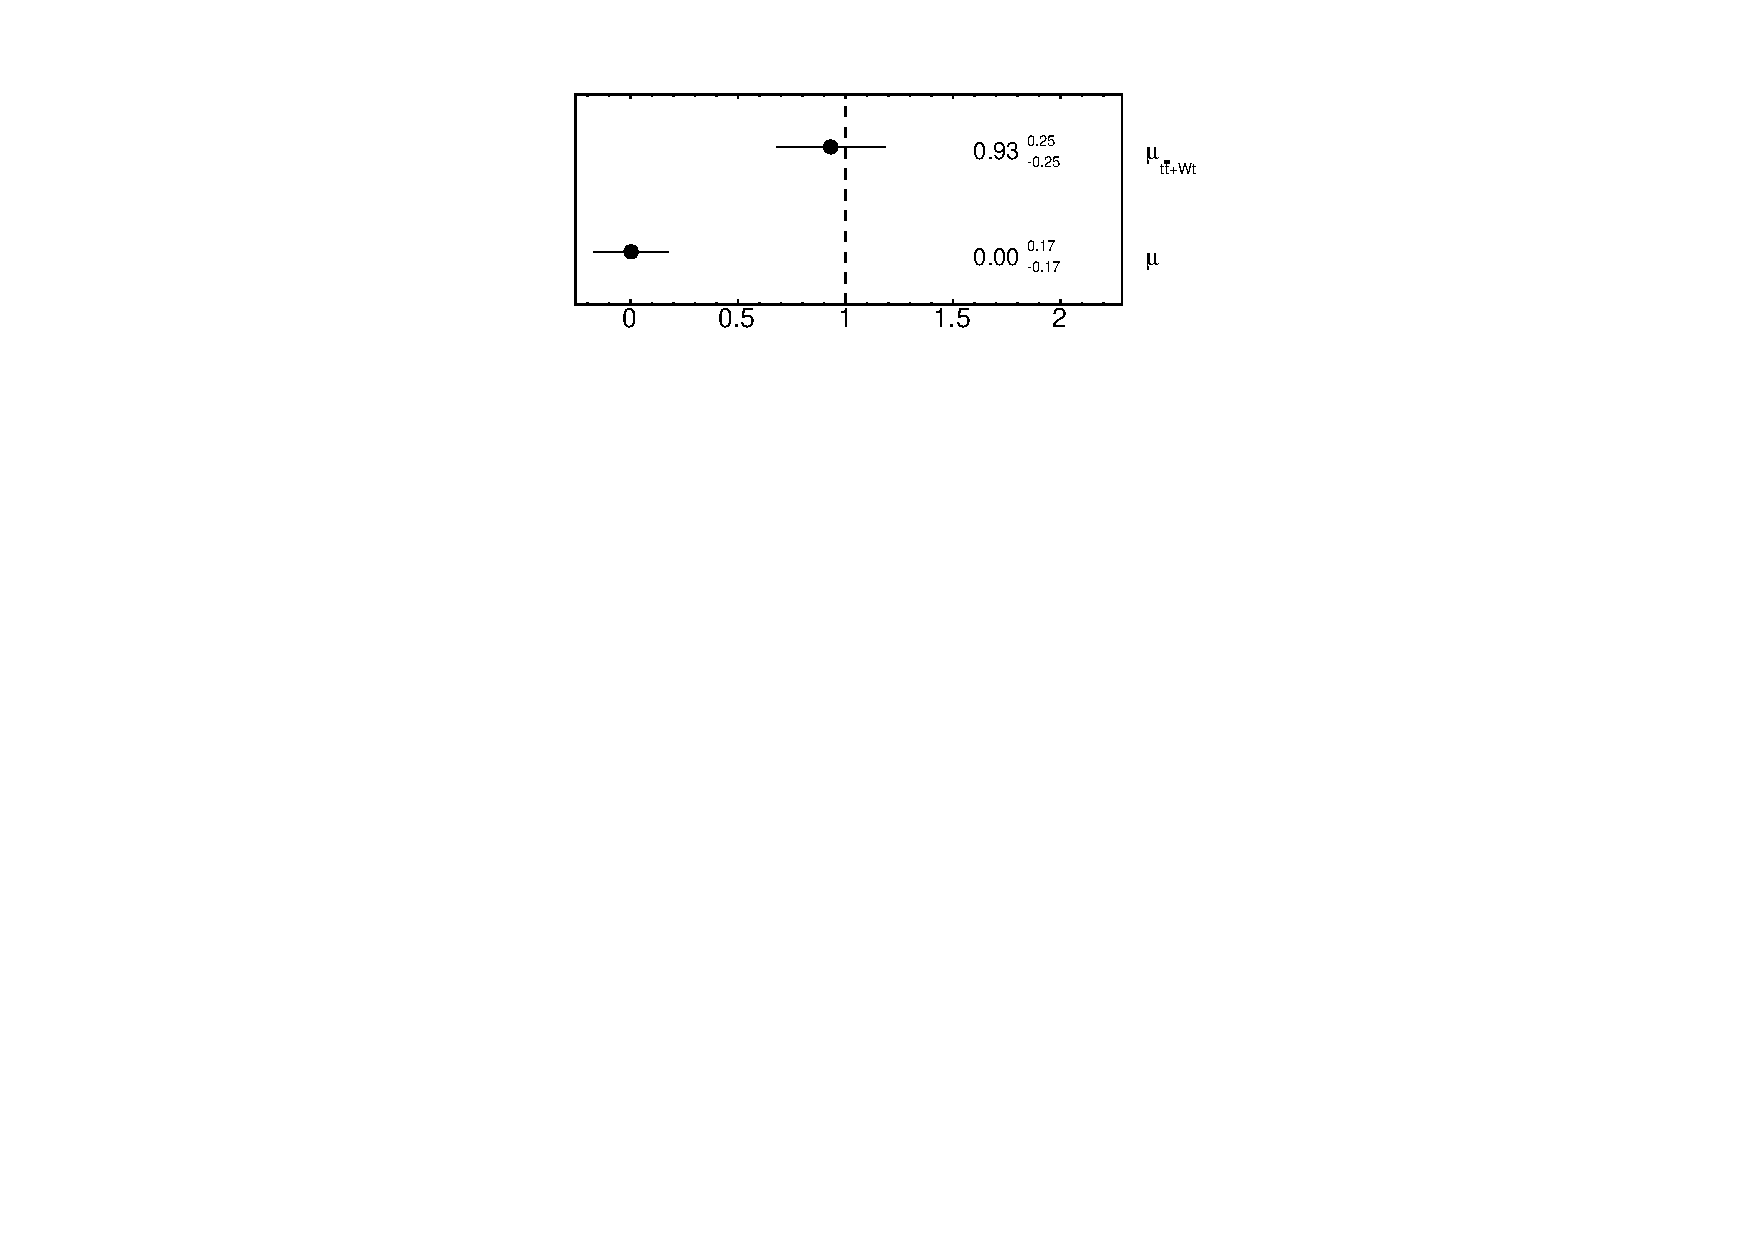
\includegraphics[width=.6\textwidth]{Chapters/CH8/figures/SPLUSB_CRSR_UsingDL1rcFullSys/NormFactors}
	\caption{Normalisation factors for the S+B \tZc fit in SRs+CRs with realistic Asimov.}%
	\label{fig:stat:tzc:splusb:crsr:norm}
\end{figure}

\begin{figure}[htbp]
	\centering
	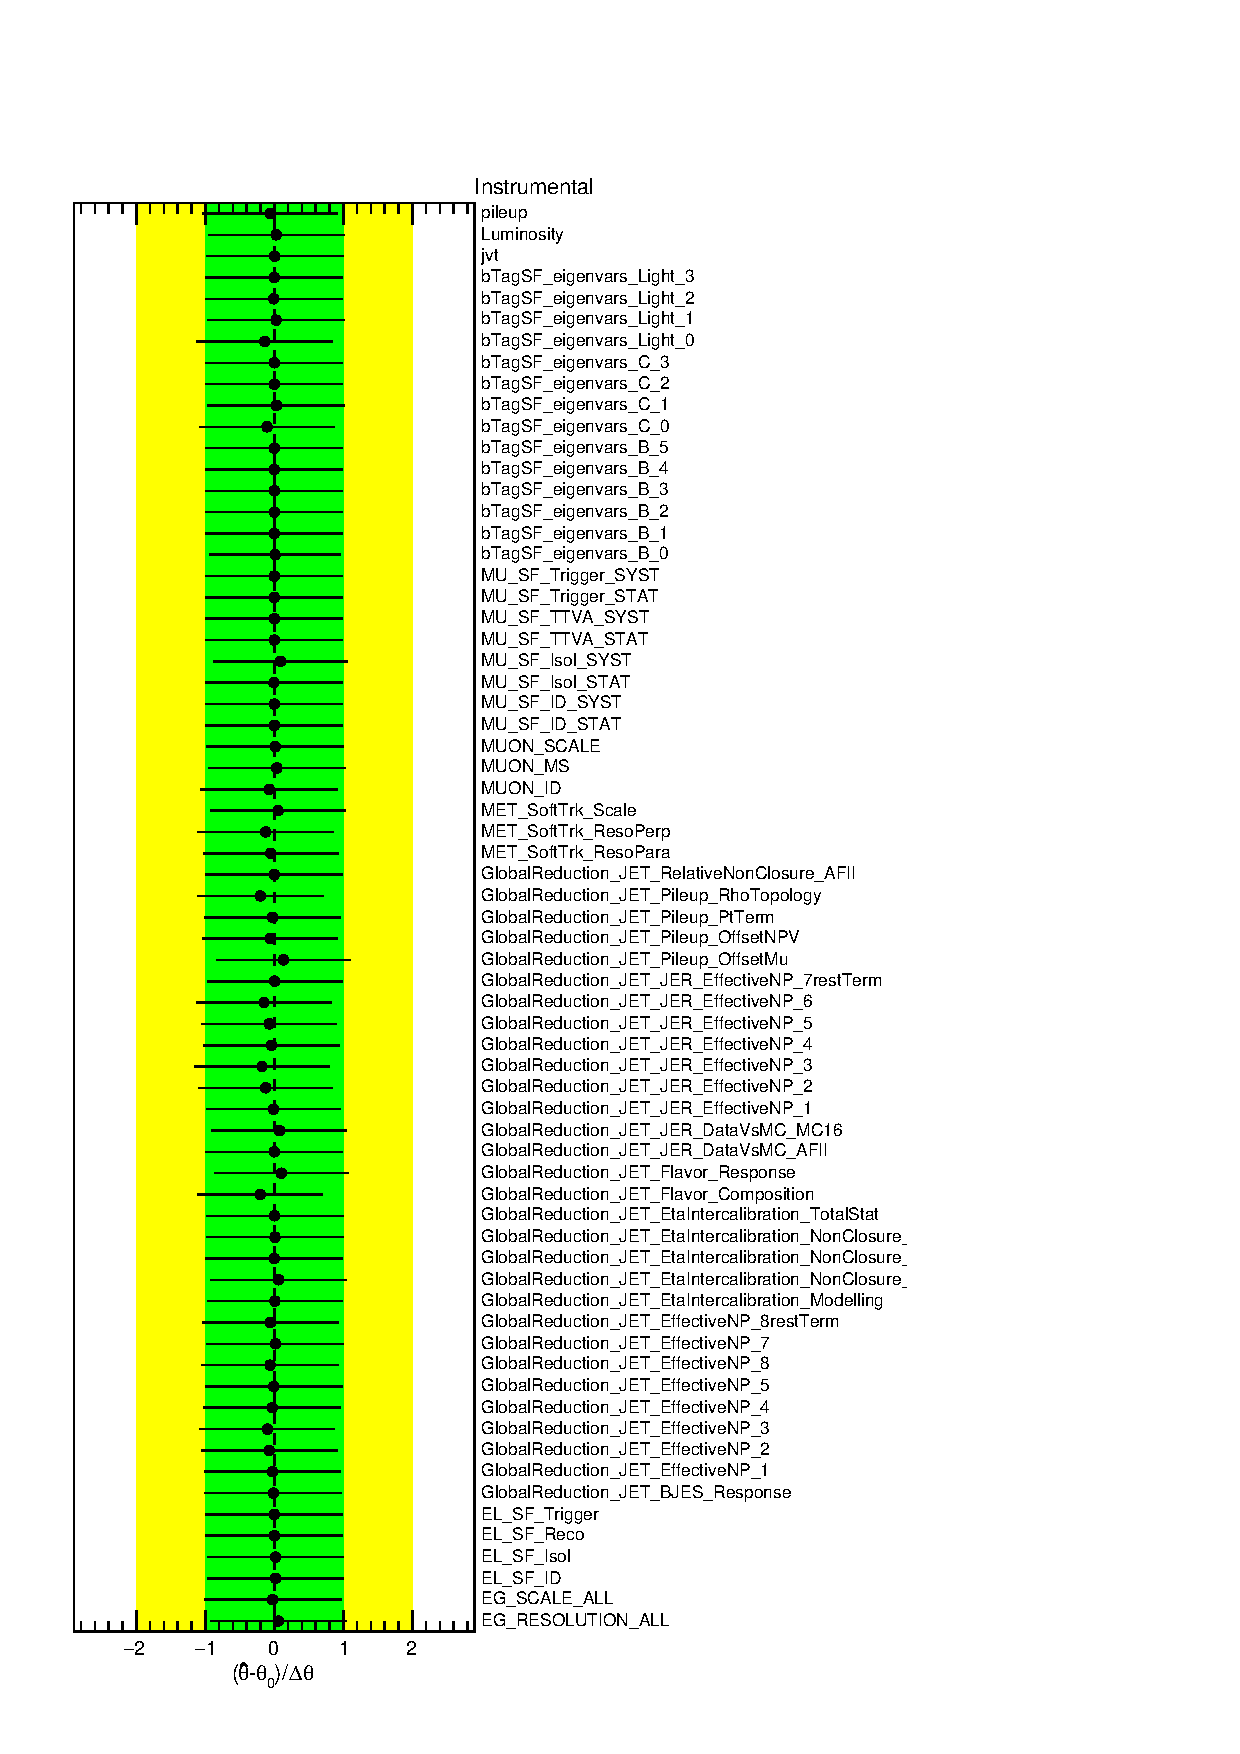
\includegraphics[width=.8\textwidth]{Chapters/CH8/figures/SPLUSB_CRSR_UsingDL1rcFullSys/NuisPar_Instrumental}
	\caption{Pulls and constraints of the instrumental nuisance parameters for the S+B \tZc fit in SRs+CRs with realistic Asimov.}%
	\label{fig:stat:tzc:splusb:crsr:np:instr}
\end{figure}

\begin{figure}[htbp]
	\centering
	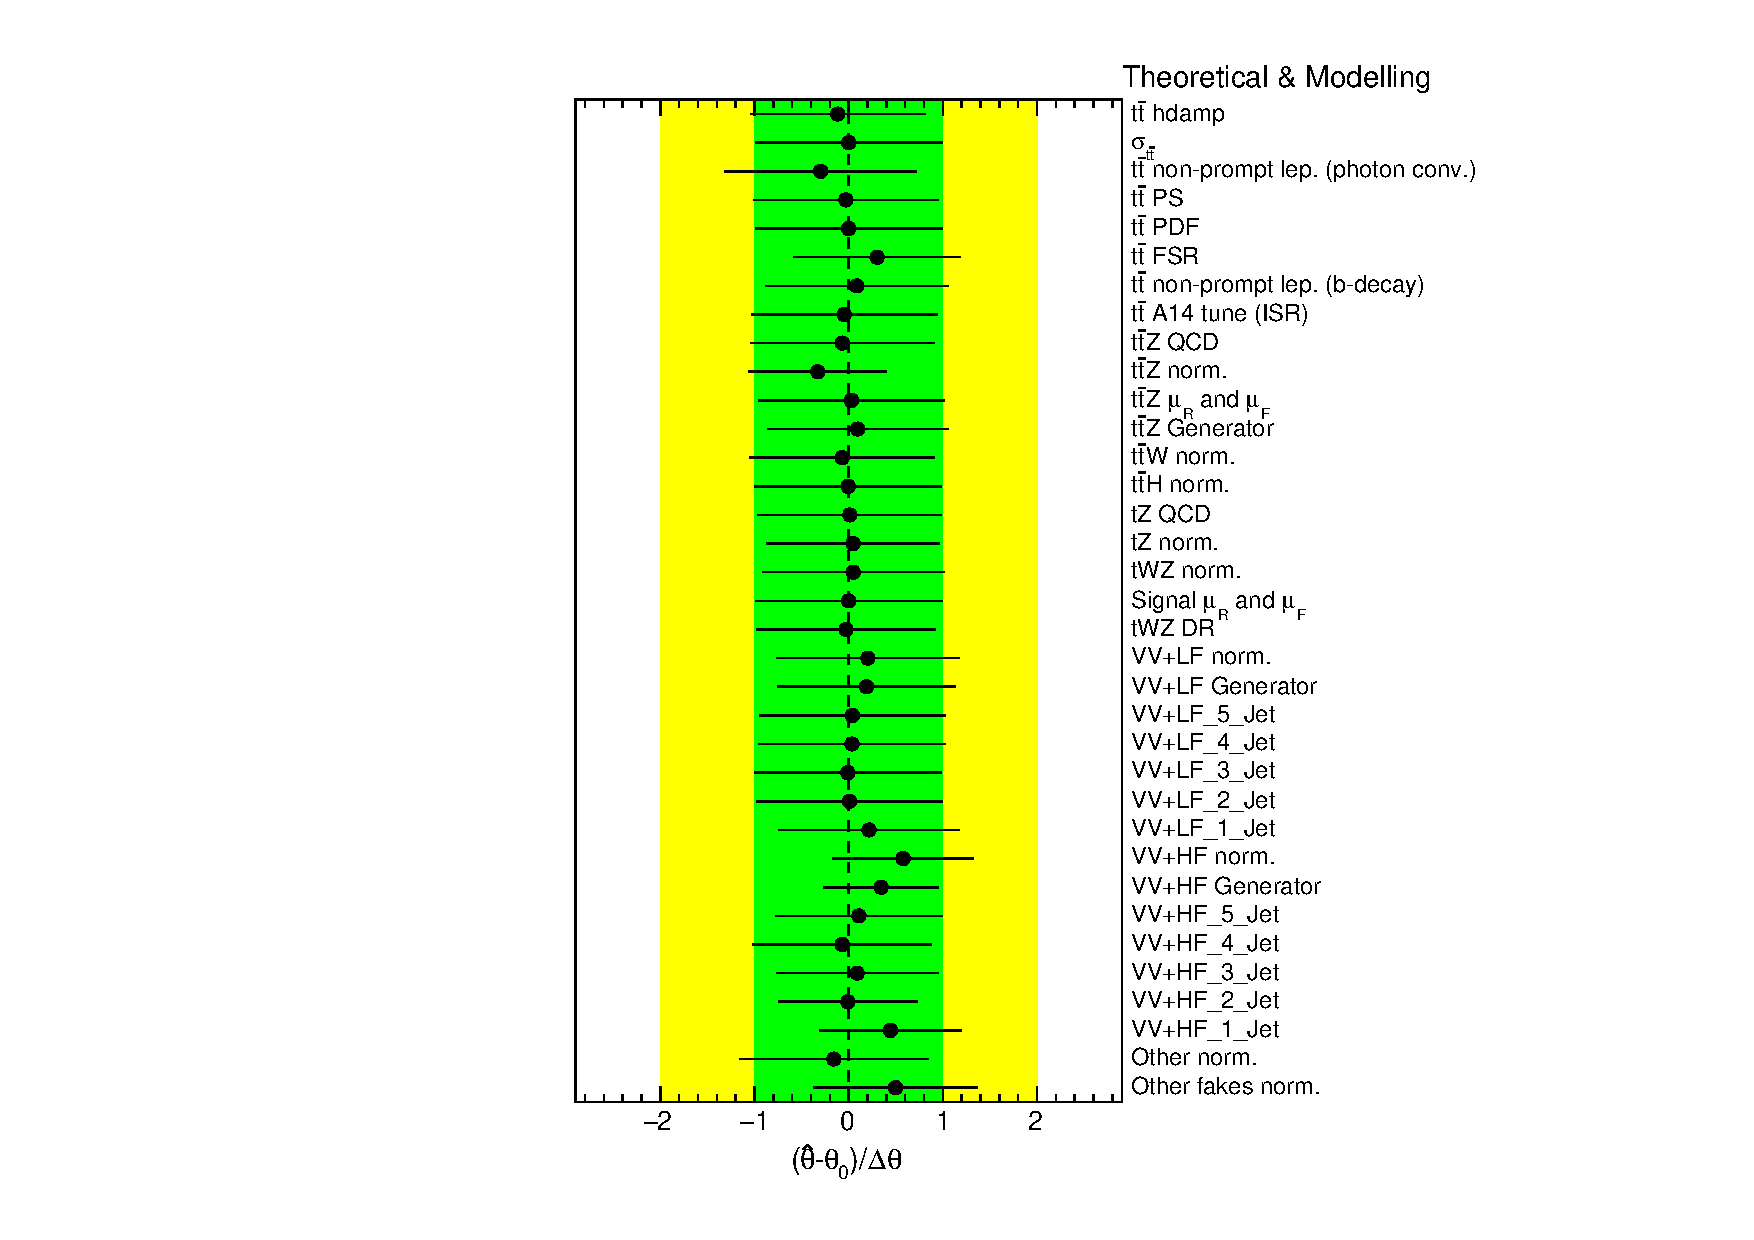
\includegraphics[width=.85\textwidth]{Chapters/CH8/figures/SPLUSB_CRSR_UsingDL1rcFullSys/NuisPar_Theoretical_&_Modelling}
	\caption{Pulls and constraints of the theoretical and modeling nuisance parameters for the S+B \tZc fit in SRs+CRs with realistic Asimov.}%
	\label{fig:stat:tzc:splusb:crsr:np:model}
\end{figure}

\begin{figure}[htbp]
	\centering
	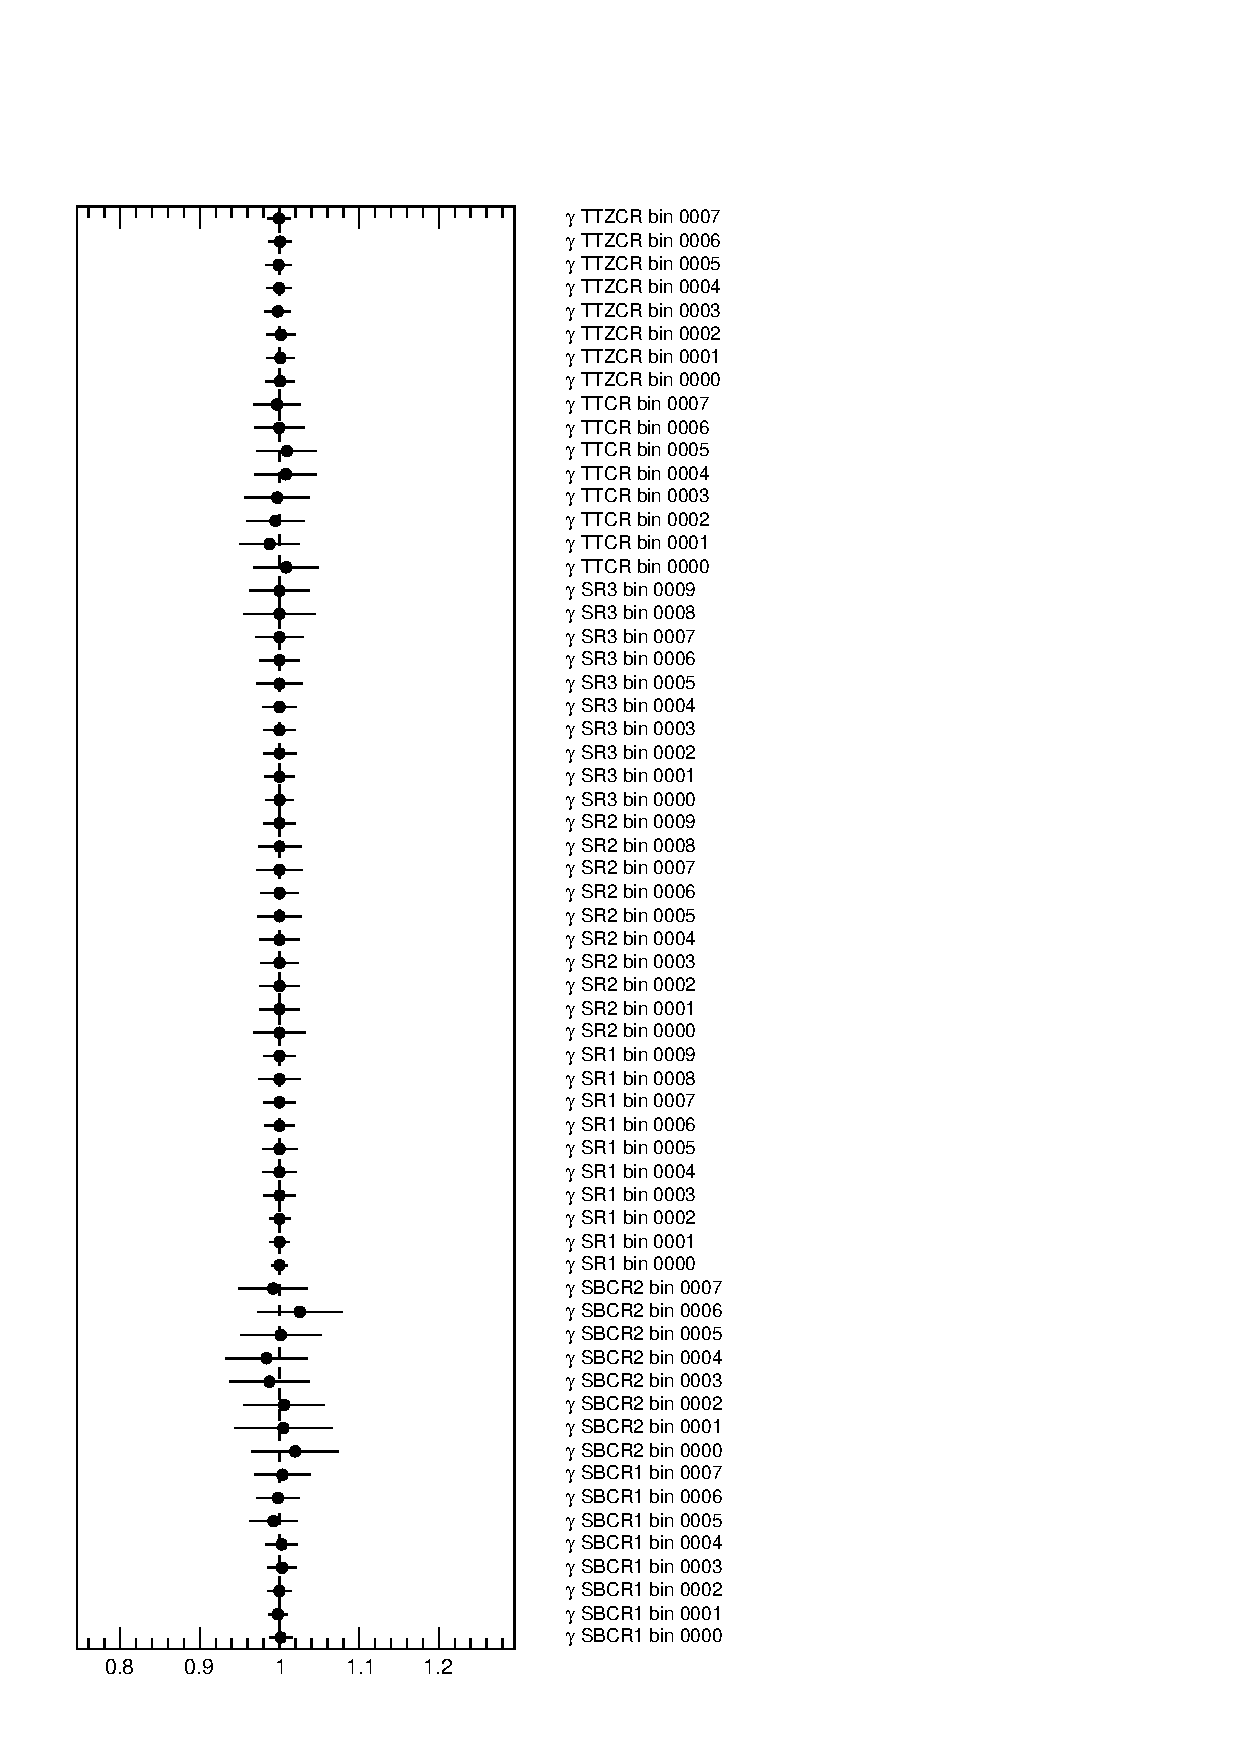
\includegraphics[width=.85\textwidth]{Chapters/CH8/figures/SPLUSB_CRSR_UsingDL1rcFullSys/Gammas}
	\caption{Gamma parameters for the S+B \tZc fit in SRs+CRs with realistic Asimov.}%
	\label{fig:stat:tzc:splusb:crsr:gamma}
\end{figure}

\begin{figure}[htbp]
	\centering
	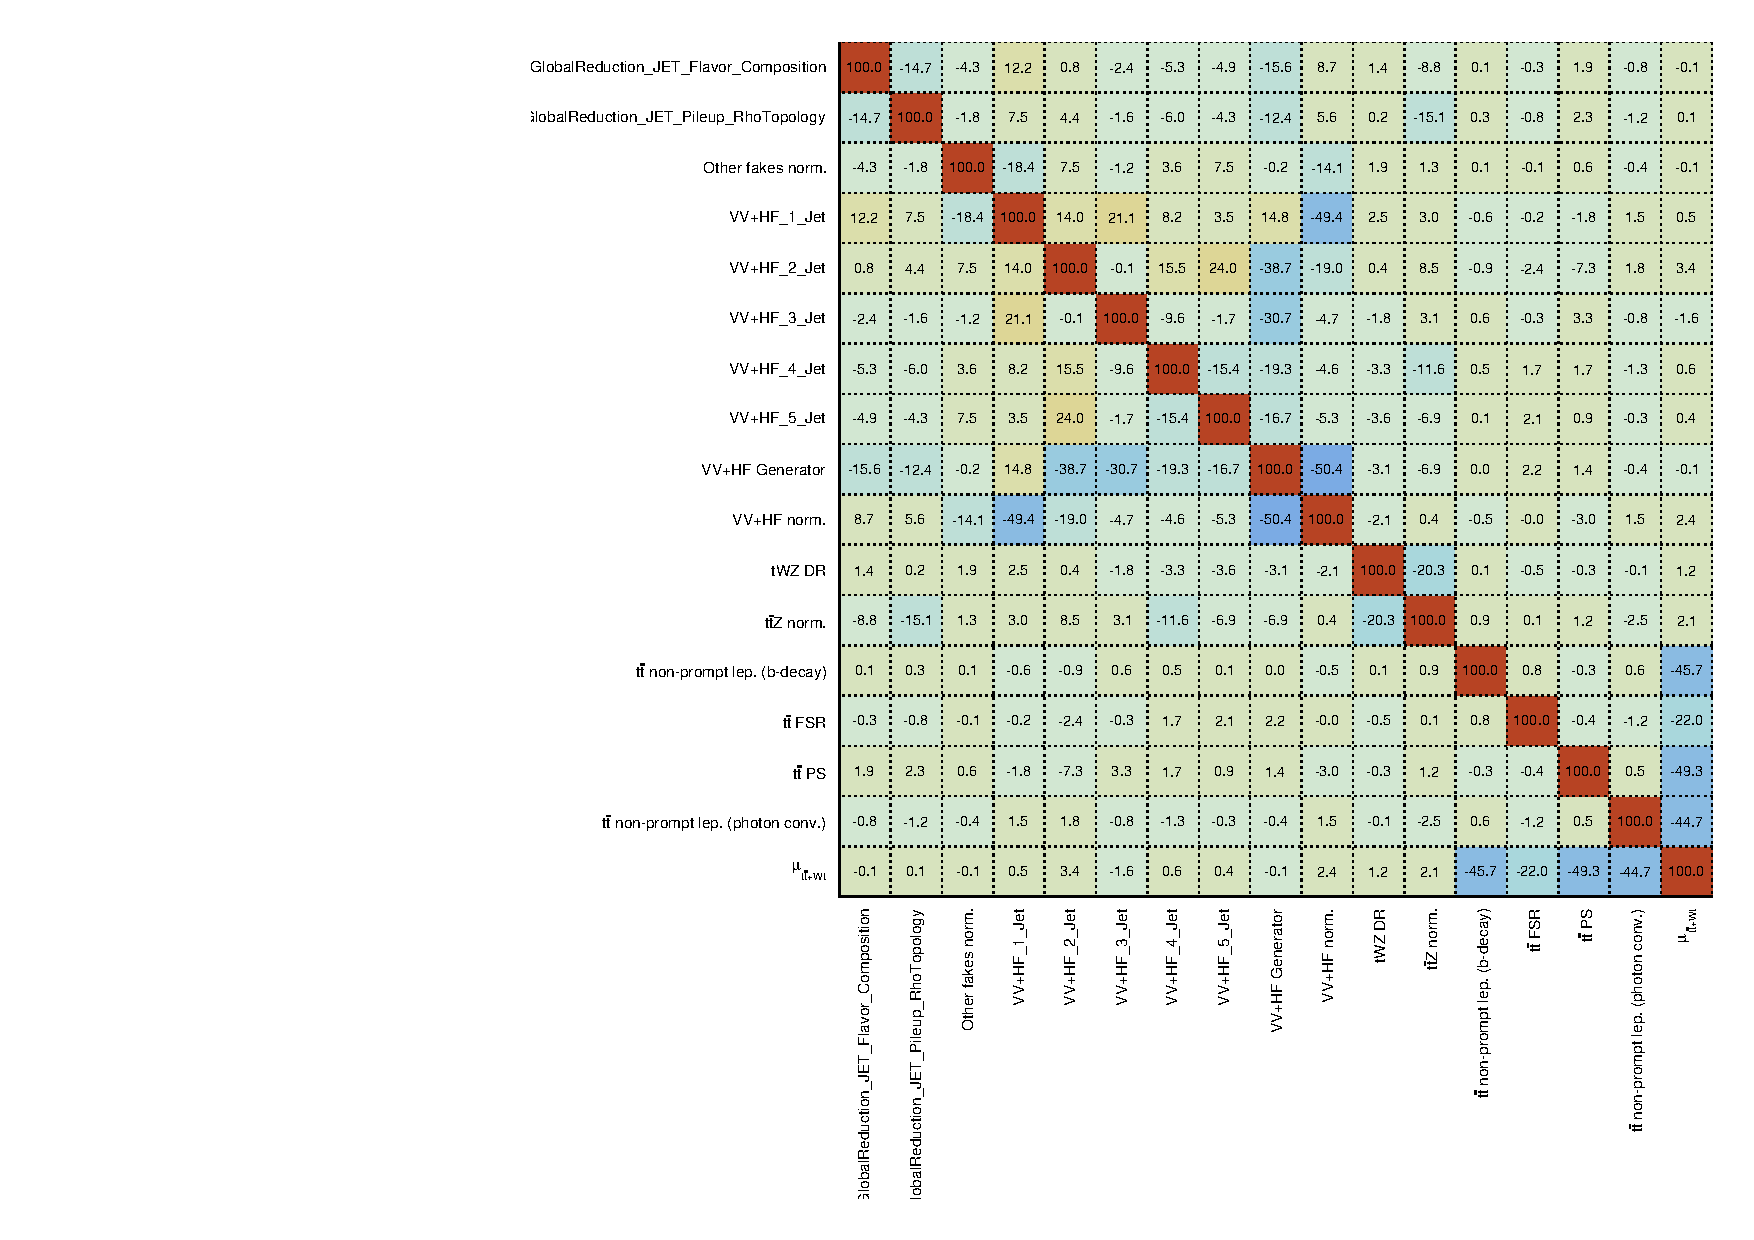
\includegraphics[width=.95\textwidth]{Chapters/CH8/figures/SPLUSB_CRSR_UsingDL1rcFullSys/CorrMatrix}
	\caption{Correlation matrix of the nuisance paramenters for the S+B \tZc fit in SRs+CRs with realistic Asimov.}%
	\label{fig:stat:tzc:splusb:crsr:corrmatrix}
\end{figure}

\begin{figure}[htbp]
	\centering
	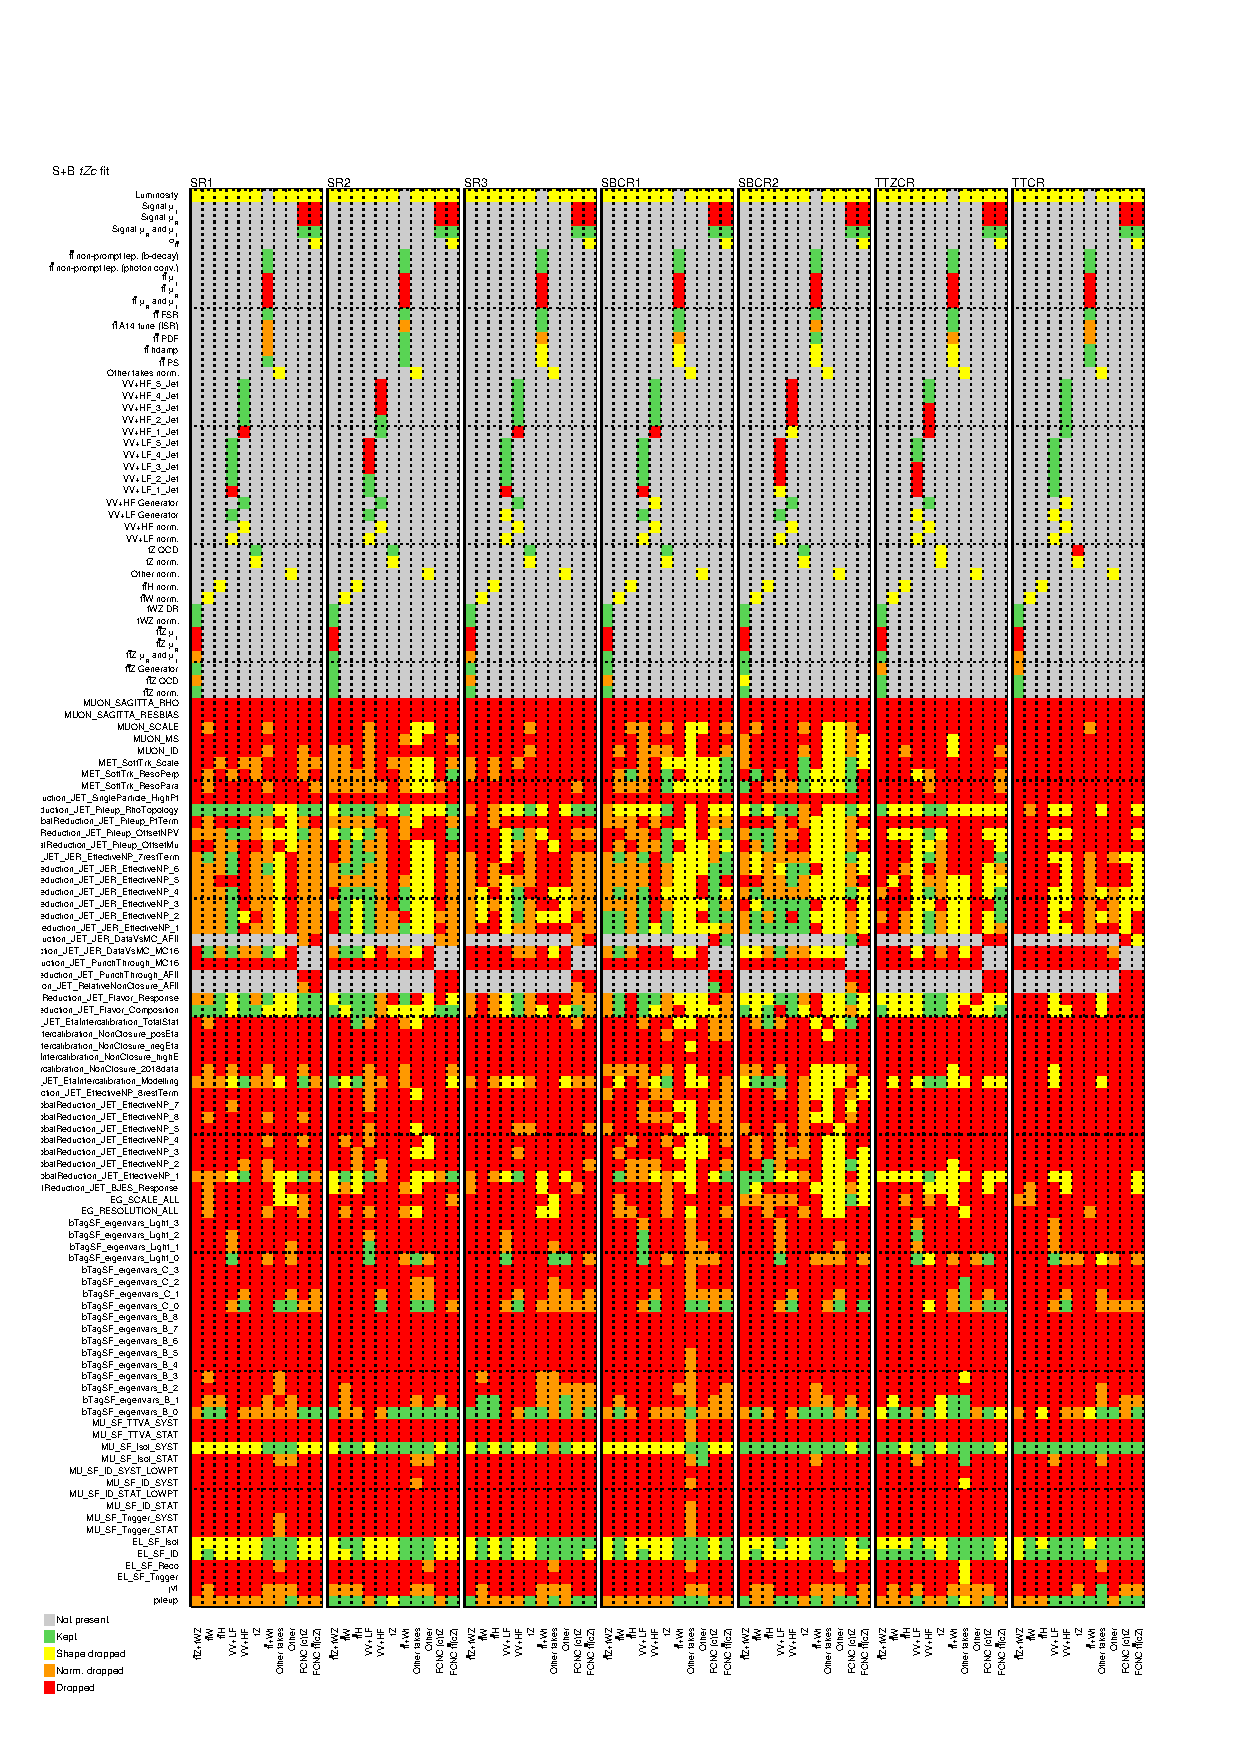
\includegraphics[width=.85\textwidth]{Chapters/CH8/figures/SPLUSB_CRSR_UsingDL1rcFullSys/Pruning}
	\caption{Pruning of the nuisance parameters for the S+B \tZc fit in SRs+CRs with realistic Asimov.}%
	\label{fig:stat:tzc:splusb:crsr:pruning}
\end{figure}

\begin{figure}[htbp]
	\centering
	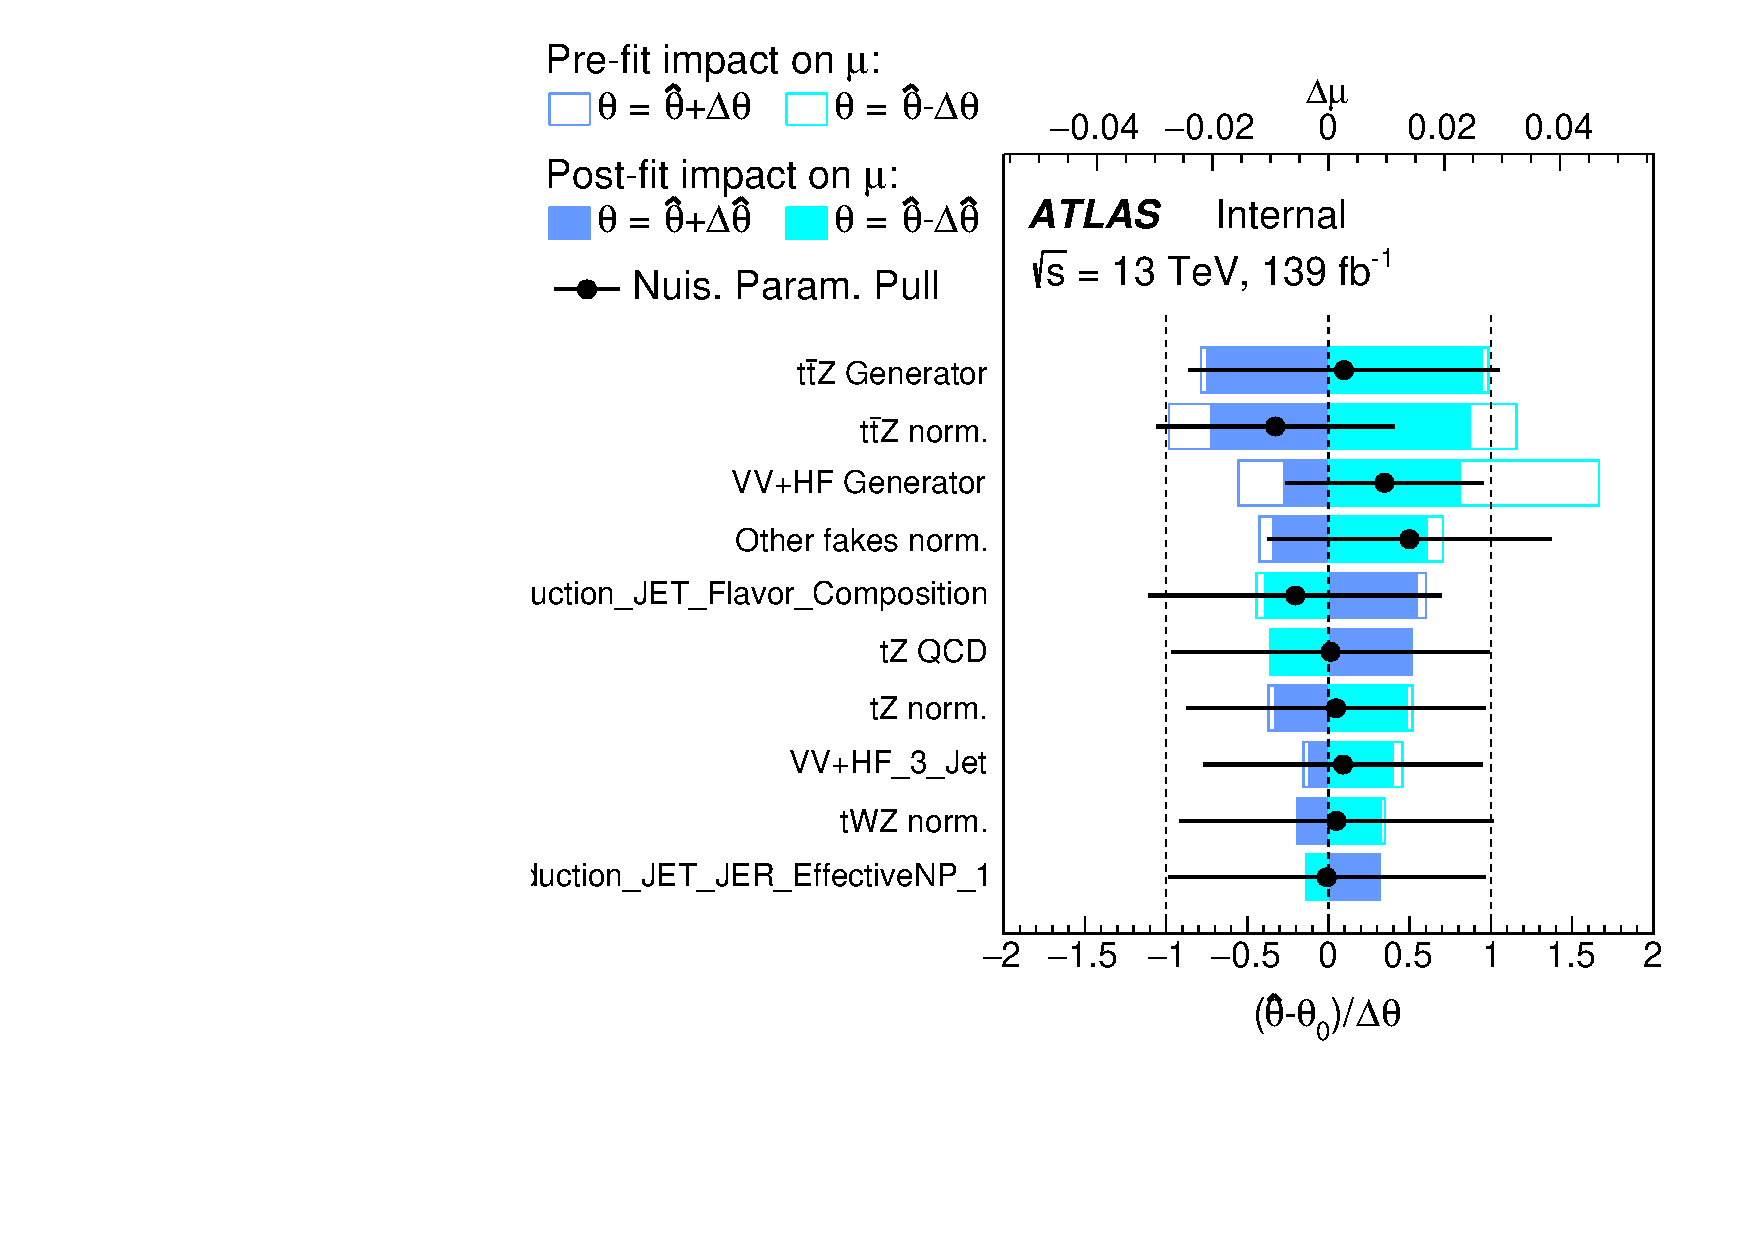
\includegraphics[width=.85\textwidth]{Chapters/CH8/figures/SPLUSB_CRSR_UsingDL1rcFullSys/Ranking}
	\caption{Ranking of the nuisance parameters for the S+B \tZc fit in SRs+CRs with realistic Asimov.}%
	\label{fig:stat:tzc:splusb:crsr:ranking}
\end{figure}

\FloatBarrier
\clearpage
%\global\pdfpageattr\expandafter{\the\pdfpageattr/Rotate 90}
\begin{table}[]
	\centering
	\tiny
	% NB: add to main document: 
% \usepackage{siunitx} 
% \sisetup{separate-uncertainty,table-format=6.3(6)}  % hint: modify table-format to best fit your tables
\begin{tabular}{|l|S|S|S|S|S|S|S|}
\toprule  
 & {SR1} & {SR2} & {SR3} & {Side-band CR1} & {Side-band CR2} & {\ttZ CR} & {\ttbar CR}\\
\midrule 
  \ttZ+\tWZ   & 168 \pm 22 & 33 \pm 7 & 82 \pm 11 & 88 \pm 12 & 9.1 \pm 2.1 & 164 \pm 22 & 14.8 \pm 1.9 \\ 
  \ttW   & 5.8 \pm 1.0 & 3.3 \pm 0.6 & 2.04 \pm 0.35 & 4.3 \pm 0.7 & 2.5 \pm 0.5 & 2.3 \pm 0.5 & 27 \pm 4 \\ 
  \ttH   & 6.1 \pm 1.0 & 0.88 \pm 0.18 & 2.6 \pm 0.4 & 2.3 \pm 0.4 & 0.36 \pm 0.07 & 5.4 \pm 0.9 & 13.8 \pm 2.1 \\ 
  \VVLF   & 28 \pm 17 & 35 \pm 13 & 2.9 \pm 2.0 & 25 \pm 15 & 18 \pm 7 & 0.20 \pm 0.22 & 0.40 \pm 0.21 \\ 
  \VVHF   & 140 \pm 100 & 160 \pm 70 & 30 \pm 22 & 130 \pm 80 & 69 \pm 28 & 13 \pm 11 & 2.3 \pm 1.4 \\ 
  \tZq   & 47 \pm 7 & 110 \pm 18 & 13.8 \pm 2.3 & 20 \pm 4 & 9.9 \pm 1.7 & 14.6 \pm 2.9 & 0.90 \pm 0.15 \\ 
  \ttbar+Wt   & 21 \pm 4 & 32 \pm 11 & 3.7 \pm 1.0 & 10 \pm 4 & 9.1 \pm 2.7 & 3.0 \pm 1.2 & 102 \pm 24 \\ 
  Other fakes   & 10 \pm 11 & 12 \pm 12 & 1.4 \pm 1.6 & 3 \pm 5 & 10 \pm 11 & 0.00 \pm 0.06 & 0.12 \pm 0.14 \\ 
  Other   & 2.5 \pm 1.5 & 3.8 \pm 2.8 & 0.48 \pm 0.25 & 2.2 \pm 1.6 & 0.8 \pm 2.6 & 1.1 \pm 0.5 & 2.9 \pm 1.5 \\ 
  FCNC (c)tZ   & 3.24 \pm 0.26 & 11.8 \pm 0.6 & 1.21 \pm 0.09 & 1.06 \pm 0.12 & 0.83 \pm 0.09 & 0.24 \pm 0.04 & 0.083 \pm 0.012 \\ 
  FCNC \ttbar(cZ)   & 57 \pm 5 & 17.7 \pm 1.9 & 21.9 \pm 1.6 & 4.2 \pm 0.6 & 1.9 \pm 0.4 & 3.7 \pm 0.5 & 0.37 \pm 0.07 \\ 
\midrule 
  Total background  & 430 \pm 110 & 390 \pm 80 & 139 \pm 25 & 280 \pm 80 & 130 \pm 32 & 203 \pm 27 & 164 \pm 25 \\ 
\midrule 
  Data   & 488 & 452 & 150 & 331 & 169 & 197 & 156 \\ 
\midrule 
  Data / Bkg.   & 1.13 \pm 0.28 & 1.17 \pm 0.24 & 1.08 \pm 0.21 & 1.18 \pm 0.35 & 1.30 \pm 0.34 & 0.97 \pm 0.14 & 0.95 \pm 0.16 \\ 
\bottomrule 
\end{tabular} 

	\caption{Pre-fit event yields in the S+B \tZc fit in SRs+CRs with realistic Asimov. \TabErrStatSys} 
	\label{tab:stat:tzc:splusb:crsr:yields:prefit}
\end{table} 

\begin{table}[]
	\centering
	\tiny
	% NB: add to main document: 
% \usepackage{siunitx} 
% \sisetup{separate-uncertainty,table-format=6.3(6)}  % hint: modify table-format to best fit your tables
\begin{tabular}{|p{0.10\textwidth}|>{\centering}p{0.08\textwidth}|>{\centering}p{0.08\textwidth}|>{\centering}p{0.08\textwidth}|>{\centering}p{0.09\textwidth}|>{\centering}p{0.09\textwidth}|>{\centering}p{0.09\textwidth}|>{\centering\arraybackslash}p{0.09\textwidth}|}
\toprule  
 & {SR1tZc} & {SR2tZc} & {SR3tZc} & {Side-band CR1tZc} & {Side-band CR2} & {\ttZ CR} & {\ttbar CR}\\
\midrule 
 \ttZ+\tWZ   & 163 $\pm$ 14 & 34 $\pm$ 6 & 79 $\pm$ 7 & 85 $\pm$ 9 & 9.3 $\pm$ 1.9 & 157 $\pm$ 13 & 14.4 $\pm$ 1.3 \\ 
\ttW   & 5.7 $\pm$ 0.9 & 3.4 $\pm$ 0.6 & 2.01 $\pm$ 0.32 & 4.2 $\pm$ 0.7 & 2.5 $\pm$ 0.5 & 2.2 $\pm$ 0.4 & 26 $\pm$ 4 \\ 
\ttH   & 6.1 $\pm$ 0.9 & 0.90 $\pm$ 0.17 & 2.6 $\pm$ 0.4 & 2.3 $\pm$ 0.4 & 0.37 $\pm$ 0.07 & 5.3 $\pm$ 0.8 & 13.8 $\pm$ 2.1 \\ 
\VVLF   & 32 $\pm$ 18 & 39 $\pm$ 14 & 3.3 $\pm$ 2.1 & 29 $\pm$ 16 & 21 $\pm$ 8 & 0.24 $\pm$ 0.23 & 0.40 $\pm$ 0.18 \\ 
\VVHF   & 198 $\pm$ 32 & 212 $\pm$ 29 & 43 $\pm$ 7 & 172 $\pm$ 25 & 94 $\pm$ 16 & 18 $\pm$ 6 & 3.3 $\pm$ 0.5 \\ 
\tZq   & 46 $\pm$ 7 & 112 $\pm$ 16 & 13.9 $\pm$ 2.1 & 19.6 $\pm$ 3.3 & 10.1 $\pm$ 1.6 & 14.4 $\pm$ 2.5 & 0.91 $\pm$ 0.12 \\ 
\ttbar+Wt   & 18 $\pm$ 4 & 30 $\pm$ 7 & 3.2 $\pm$ 0.7 & 9.5 $\pm$ 2.8 & 8.6 $\pm$ 1.7 & 2.5 $\pm$ 0.8 & 95 $\pm$ 13 \\ 
Other fakes   & 15 $\pm$ 11 & 17 $\pm$ 13 & 2.1 $\pm$ 1.7 & 5 $\pm$ 5 & 18 $\pm$ 15 & 0.005 $\pm$ 0.009 & 0.18 $\pm$ 0.13 \\ 
Other   & 2.2 $\pm$ 1.2 & 3.7 $\pm$ 2.5 & 0.44 $\pm$ 0.23 & 1.8 $\pm$ 1.2 & 0.2 $\pm$ 0.8 & 1.0 $\pm$ 0.5 & 2.7 $\pm$ 1.4 \\ 
FCNC (c)tZ   & 0.0 $\pm$ 0.6 & 0.0 $\pm$ 2.1 & 0.00 $\pm$ 0.21 & 0.00 $\pm$ 0.18 & 0.00 $\pm$ 0.15 & 0.00 $\pm$ 0.04 & 0.000 $\pm$ 0.014 \\ 
FCNC \ttbar(cZ)   & 0 $\pm$ 10 & 0.1 $\pm$ 3.1 & 0 $\pm$ 4 & 0.0 $\pm$ 0.7 & 0.01 $\pm$ 0.33 & 0.0 $\pm$ 0.6 & 0.00 $\pm$ 0.06 \\ 
\midrule 
Total background  & 487 $\pm$ 21 & 452 $\pm$ 20 & 150 $\pm$ 7 & 328 $\pm$ 17 & 165 $\pm$ 13 & 201 $\pm$ 12 & 157 $\pm$ 12 \\ 
\midrule 
Data   & 488 & 452 & 150 & 331 & 169 & 197 & 156 \\ 
\midrule 
Data / Bkg.   & 1.00 $\pm$ 0.04 & 1.00 $\pm$ 0.04 & 1.00 $\pm$ 0.05 & 1.01 $\pm$ 0.05 & 1.02 $\pm$ 0.08 & 0.98 $\pm$ 0.06 & 0.99 $\pm$ 0.08 \\ 
\bottomrule 
\end{tabular} 

	\caption{Post-fit event yields in the S+B \tZc fit in SRs+CRs with realistic Asimov. \TabErrStatSys} 
	\label{tab:stat:tzc:splusb:crsr:yields:postfit}
\end{table} 
\clearpage
\FloatBarrier
%\global\pdfpageattr\expandafter{\the\pdfpageattr/Rotate 0}

\clearpage
\begin{figure}[htbp]
	\centering
	\begin{tabular}{cc}
		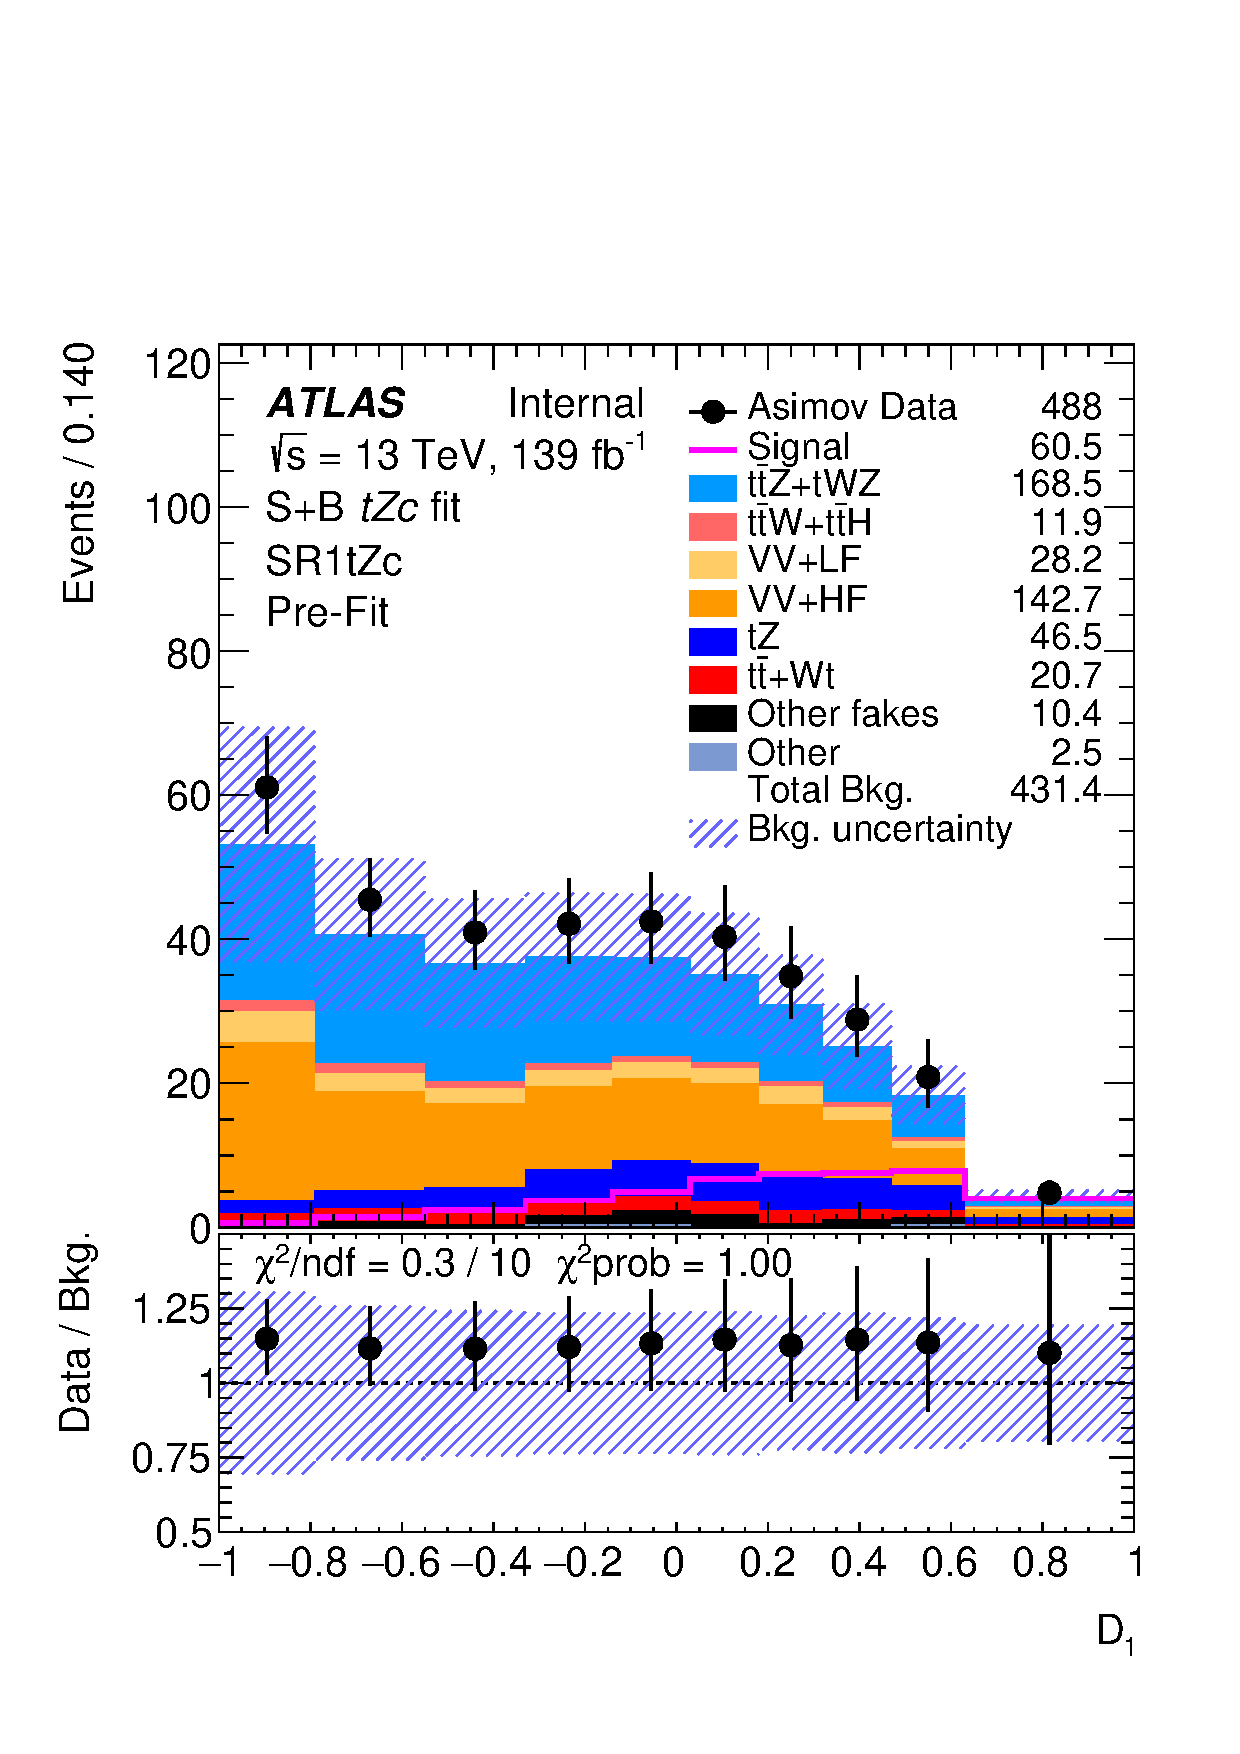
\includegraphics[width=.45\textwidth]{Chapters/CH8/figures/SPLUSB_CRSR_UsingDL1rcFullSys/Plots/SR1} &
		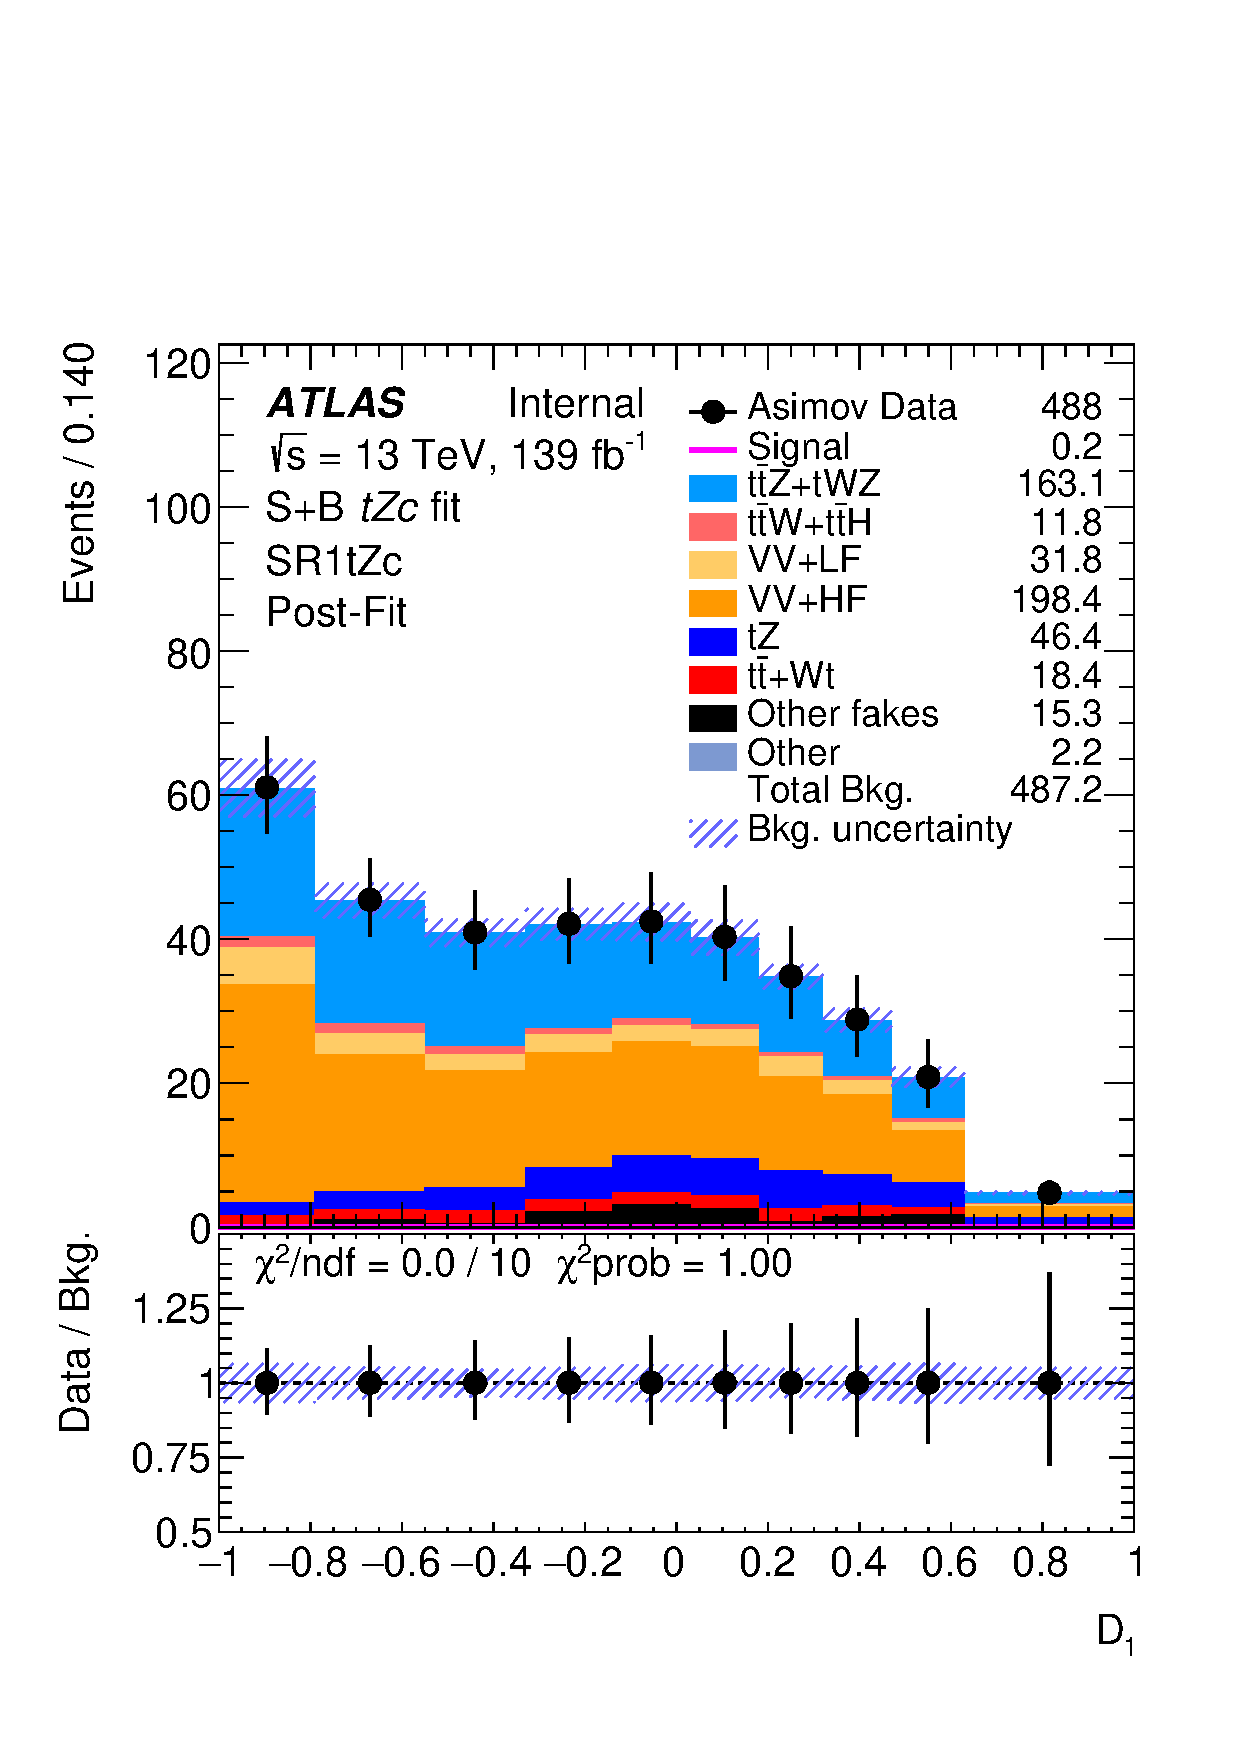
\includegraphics[width=.45\textwidth]{Chapters/CH8/figures/SPLUSB_CRSR_UsingDL1rcFullSys/Plots/SR1_postFit} \\
		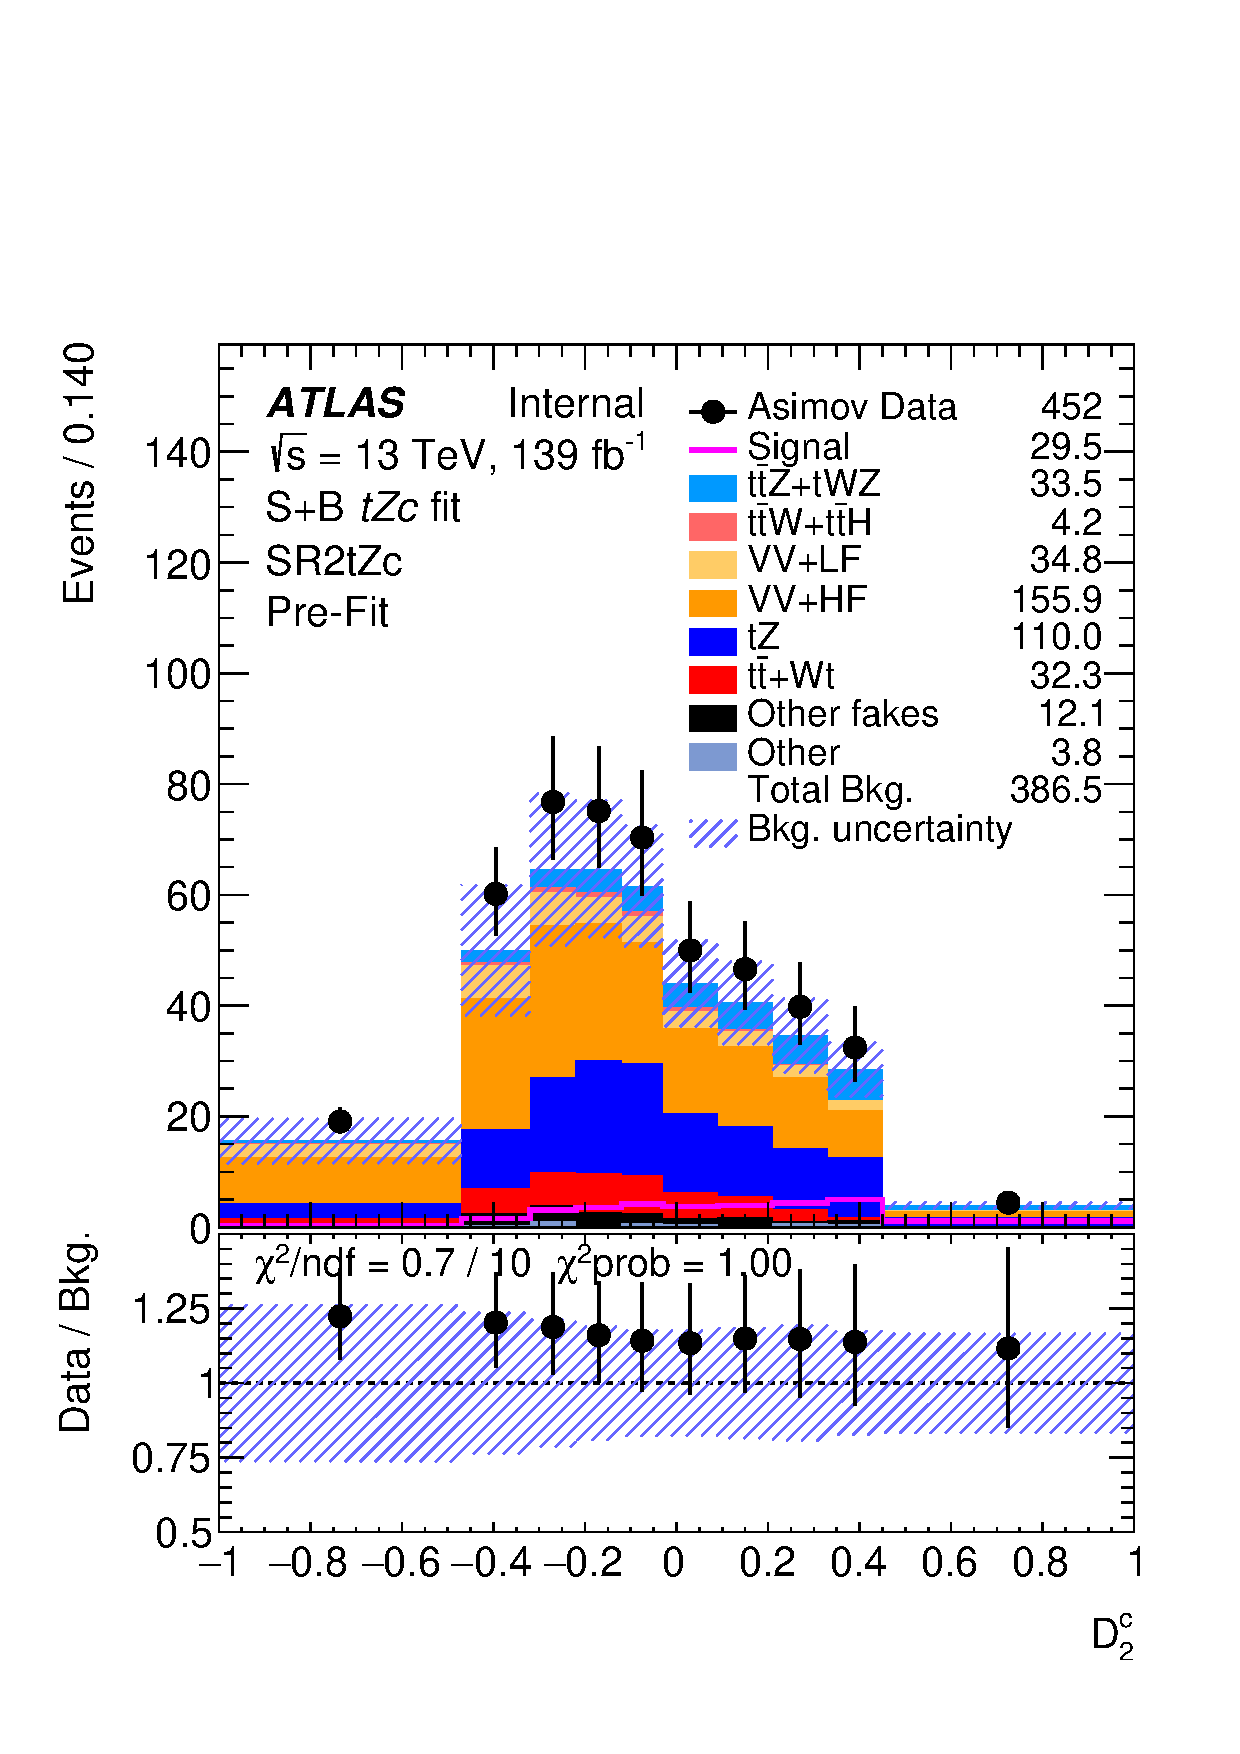
\includegraphics[width=.45\textwidth]{Chapters/CH8/figures/SPLUSB_CRSR_UsingDL1rcFullSys/Plots/SR2} &
		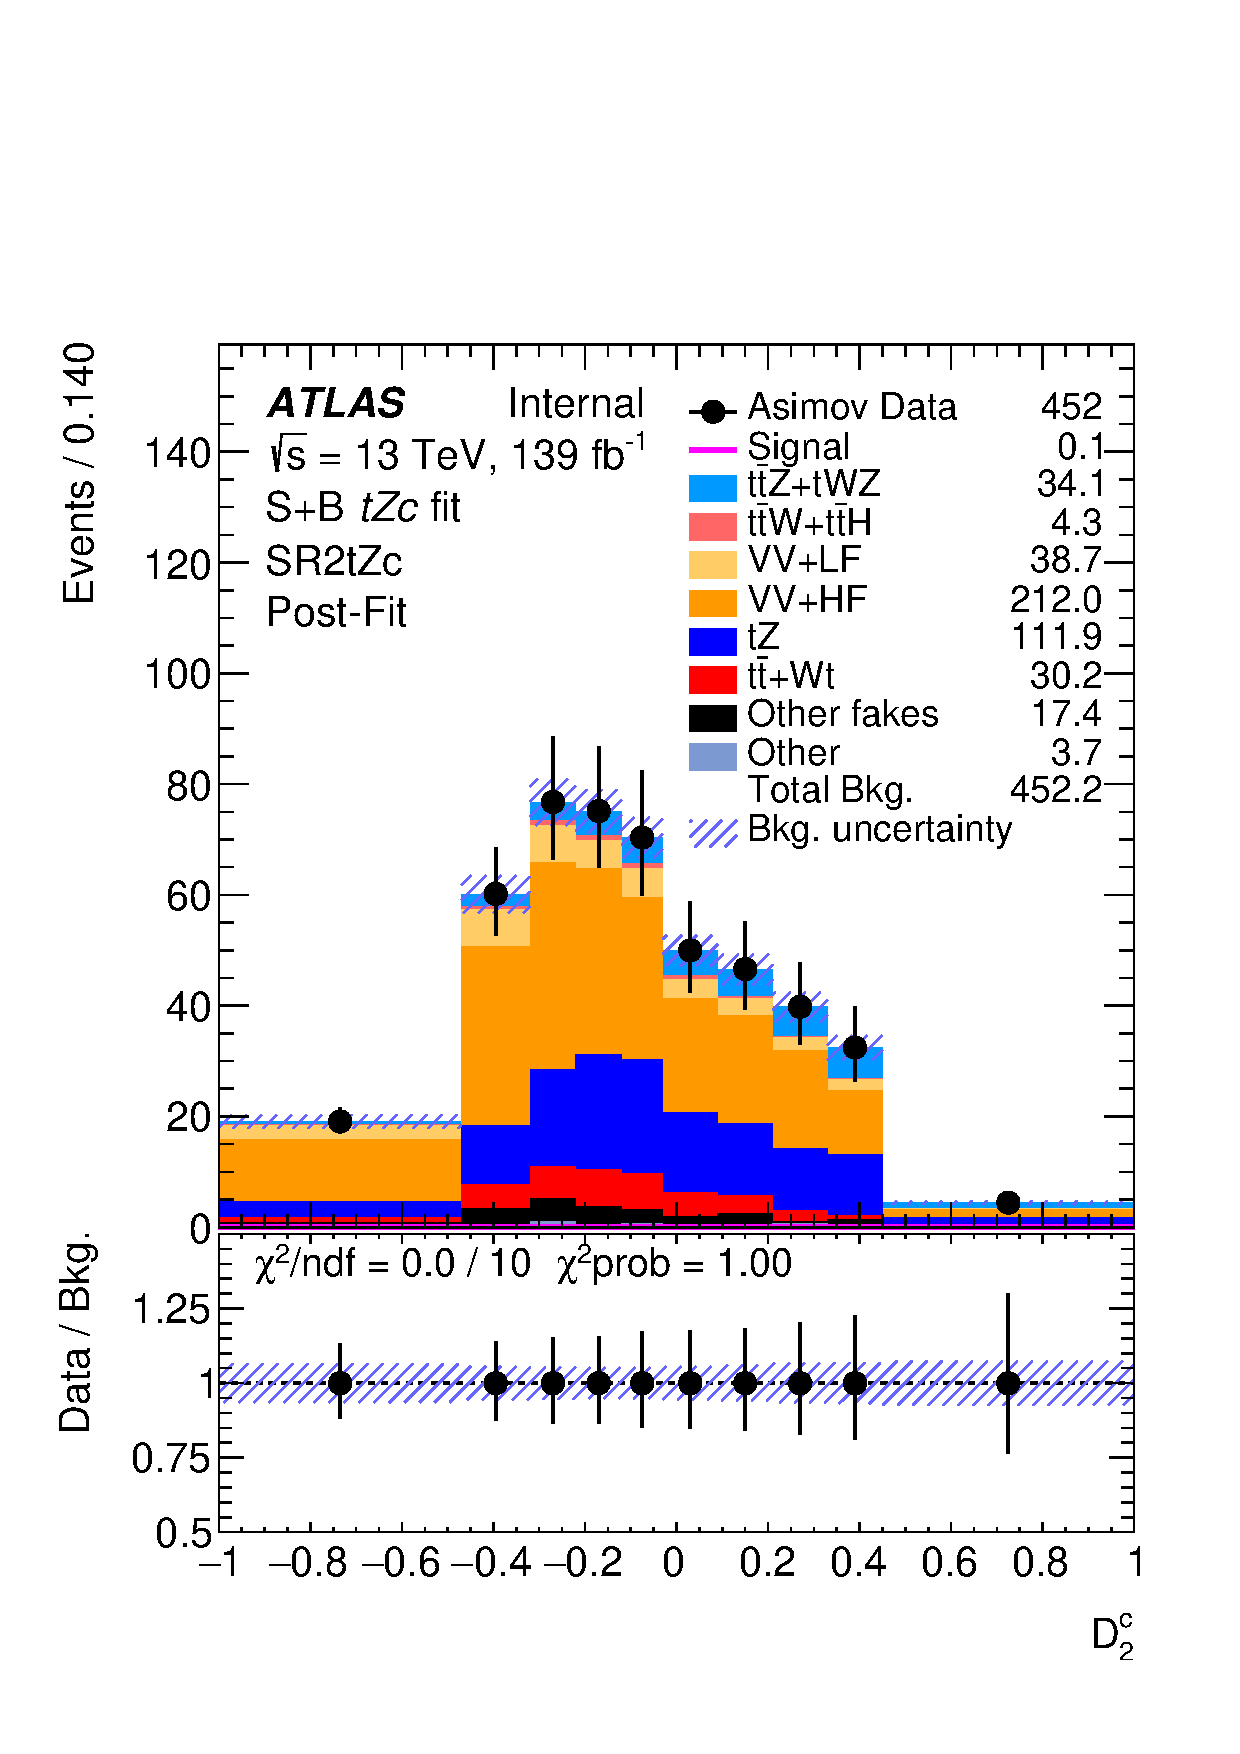
\includegraphics[width=.45\textwidth]{Chapters/CH8/figures/SPLUSB_CRSR_UsingDL1rcFullSys/Plots/SR2_postFit} \\
	\end{tabular}
	\caption{Pre-fit (left) and post-fit (right) BDTG output distributions in SR1 and SR2 for the S+B \tZc fit in SRs+CRs with realistic Asimov.
		\ErrStatSys
	}%
	\label{fig:stat:tzc:splusb:crsr:srplots:1}
\end{figure}

\begin{figure}[htbp]
	\centering
	\begin{tabular}{cc}
		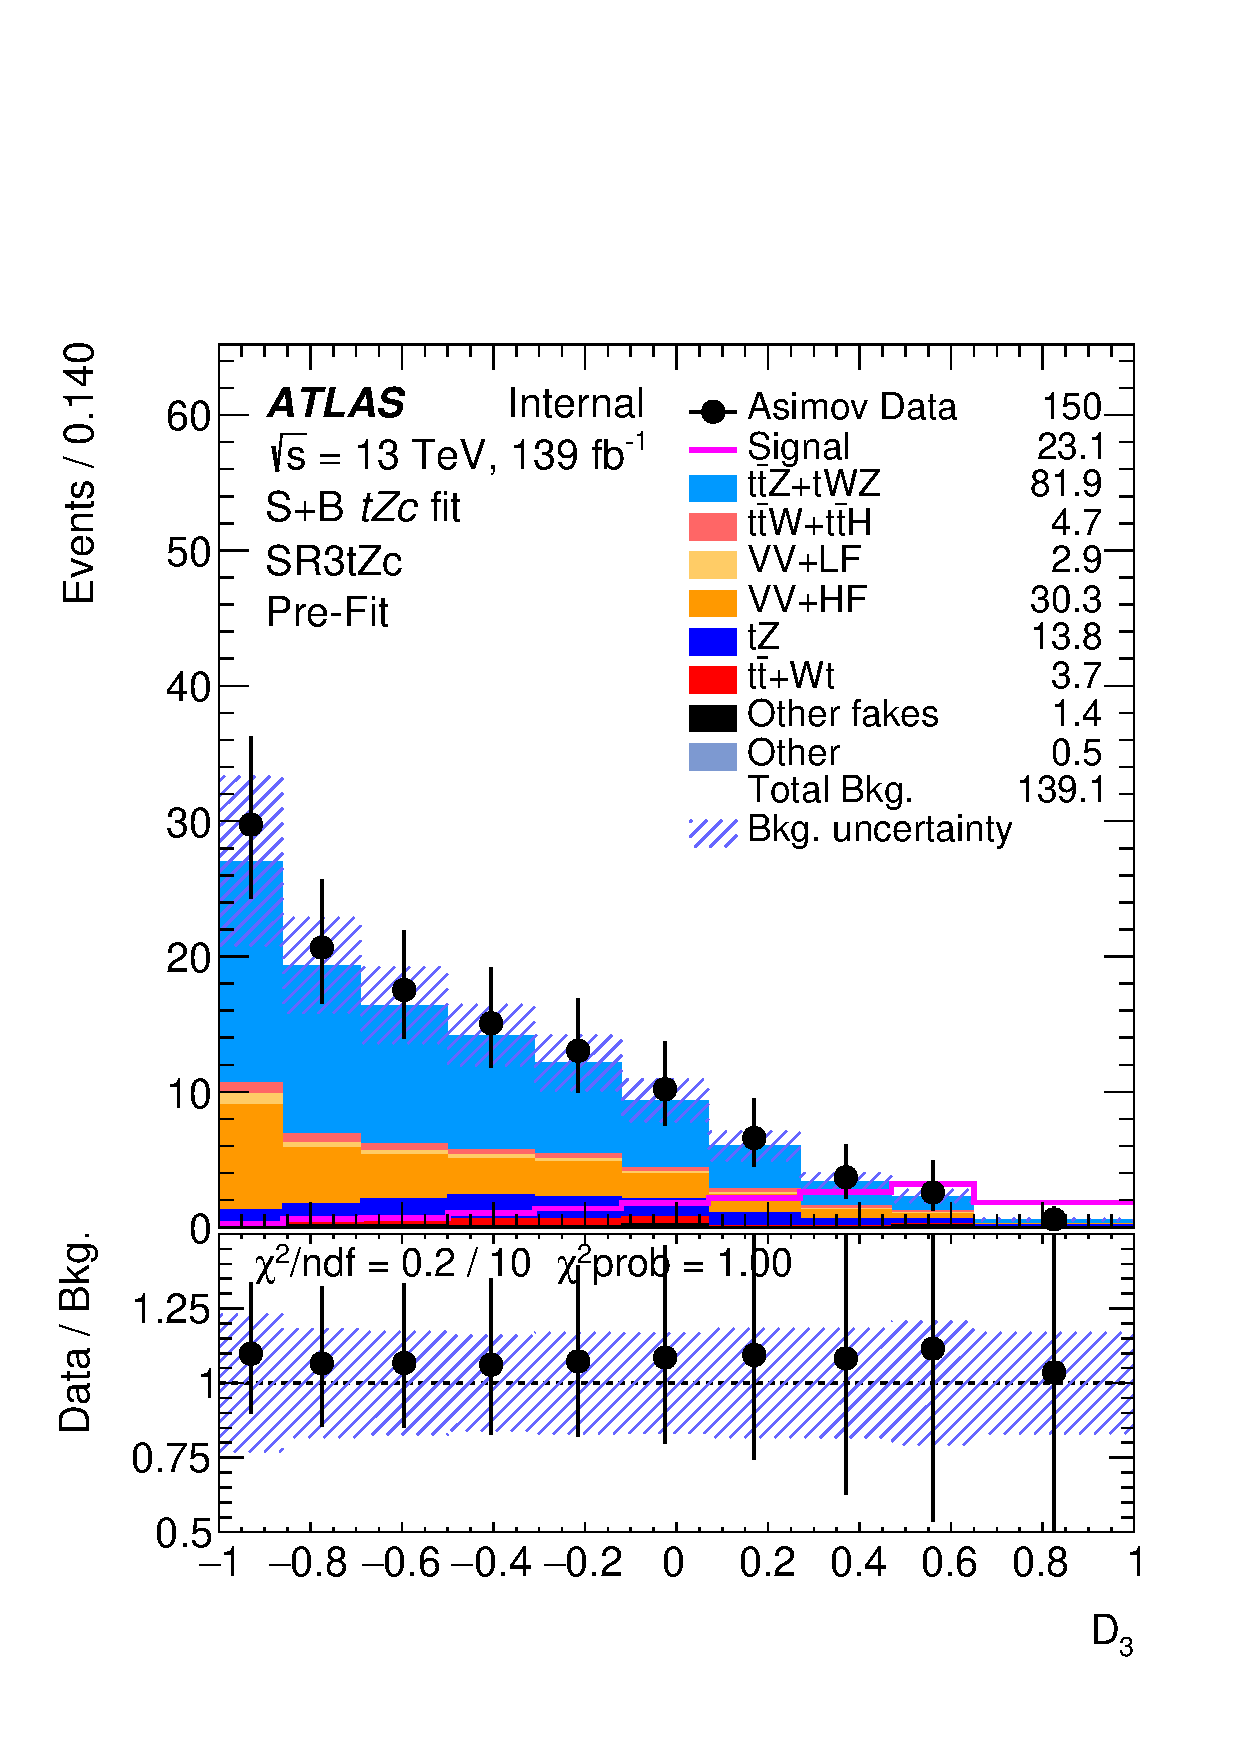
\includegraphics[width=.45\textwidth]{Chapters/CH8/figures/SPLUSB_CRSR_UsingDL1rcFullSys/Plots/SR3} &
		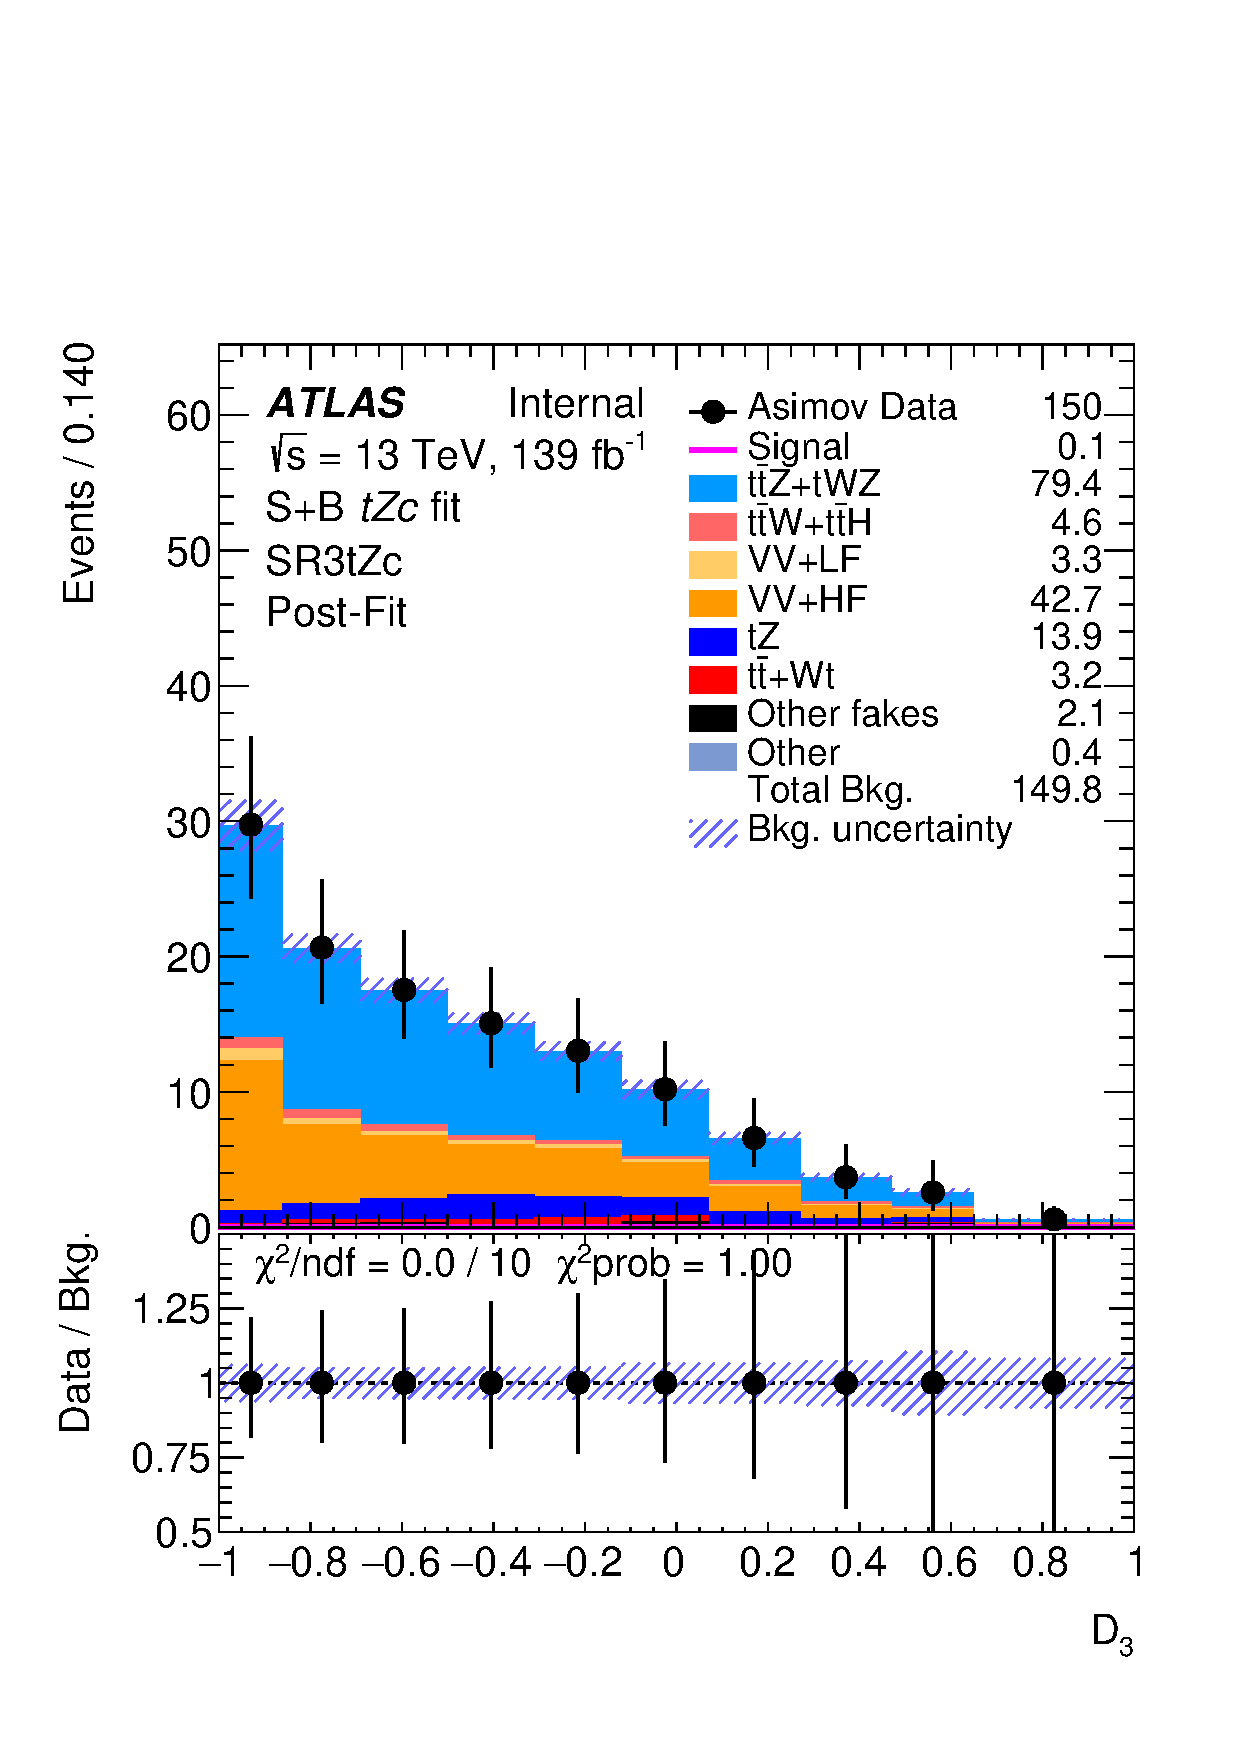
\includegraphics[width=.45\textwidth]{Chapters/CH8/figures/SPLUSB_CRSR_UsingDL1rcFullSys/Plots/SR3_postFit} \\
	\end{tabular}
	\caption{Pre-fit (left) and post-fit (right) leading lepton \pt distributions in SR3 for the S+B \tZc fit in SRs+CRs with realistic Asimov.
		\ErrStatSys
	}%
	\label{fig:stat:tzc:splusb:crsr:srplots:2}
\end{figure}

\begin{figure}[htbp]
	\centering
	\begin{tabular}{cc}
		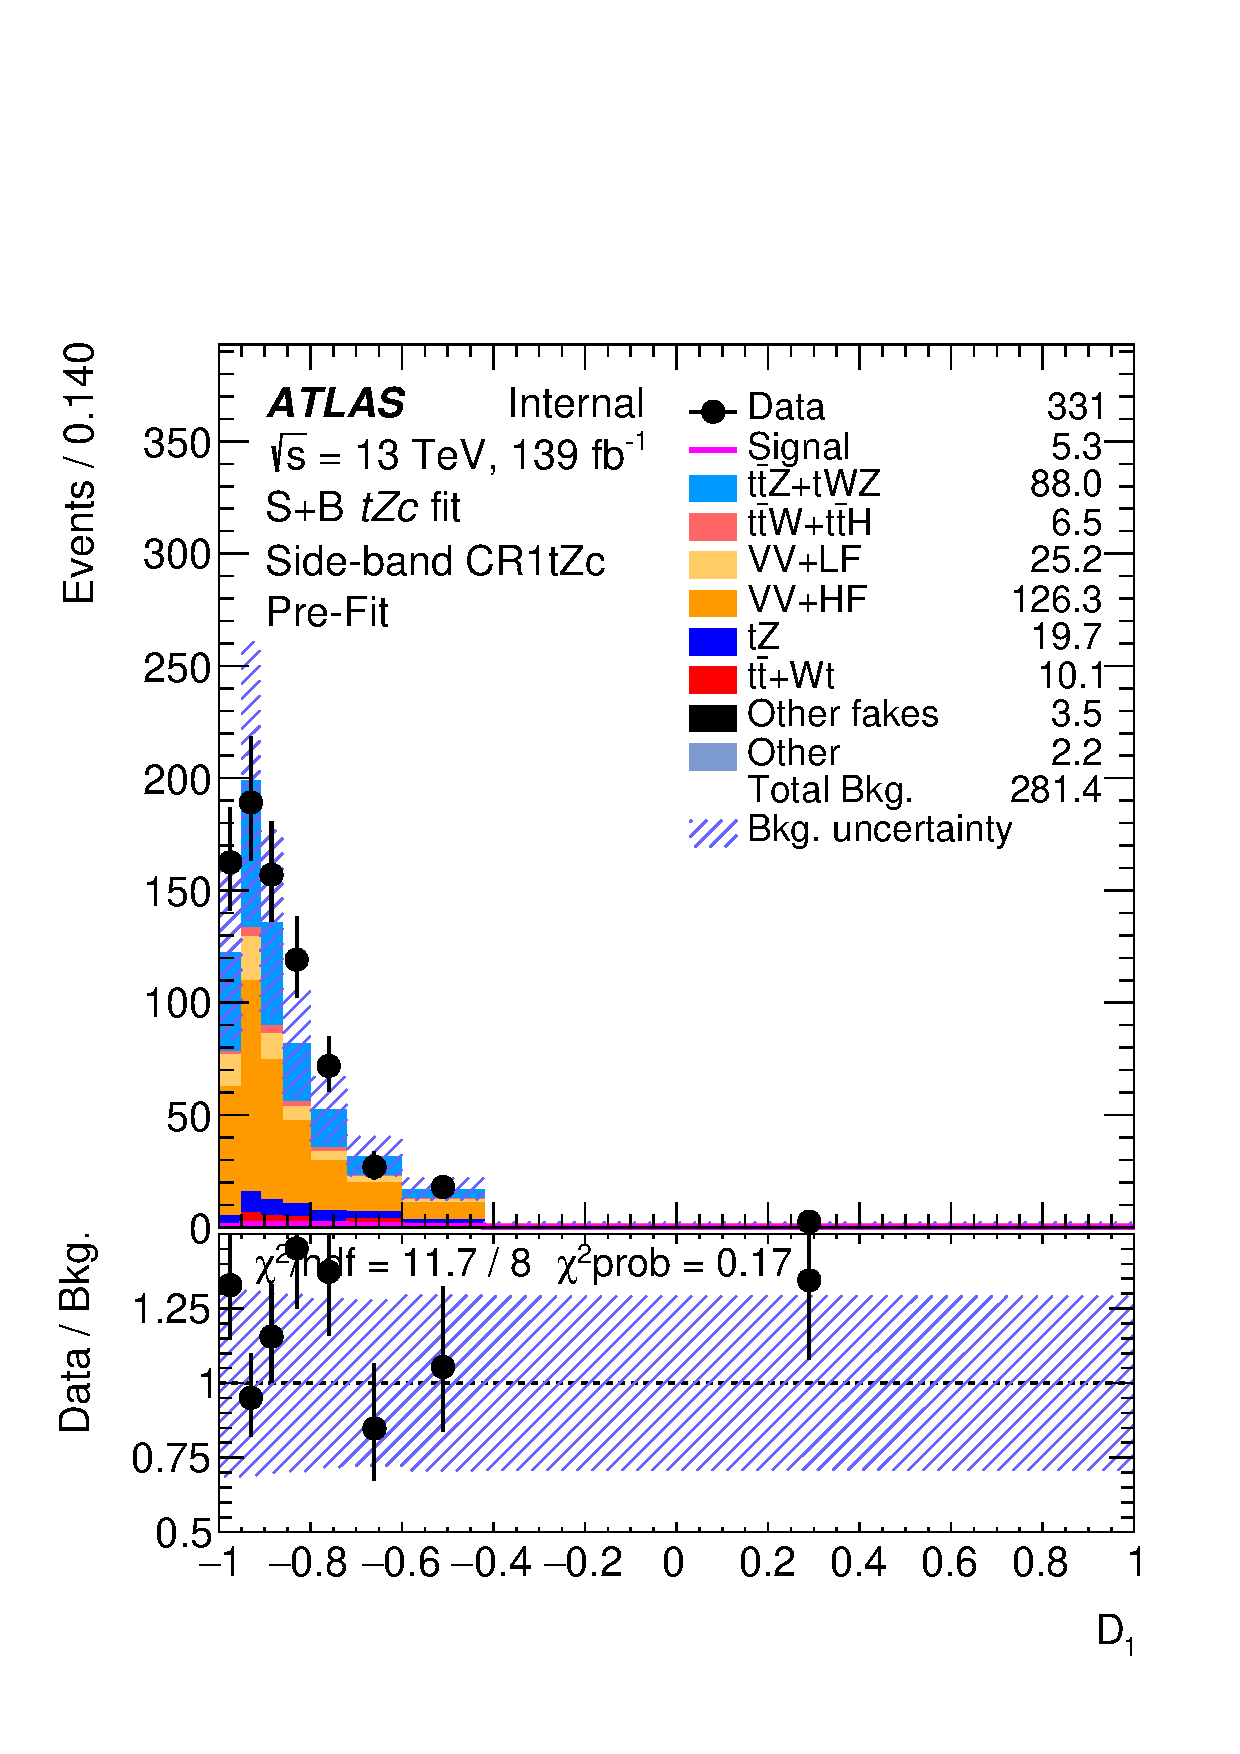
\includegraphics[width=.45\textwidth]{Chapters/CH8/figures/SPLUSB_CRSR_UsingDL1rcFullSys/Plots/SBCR1} &
		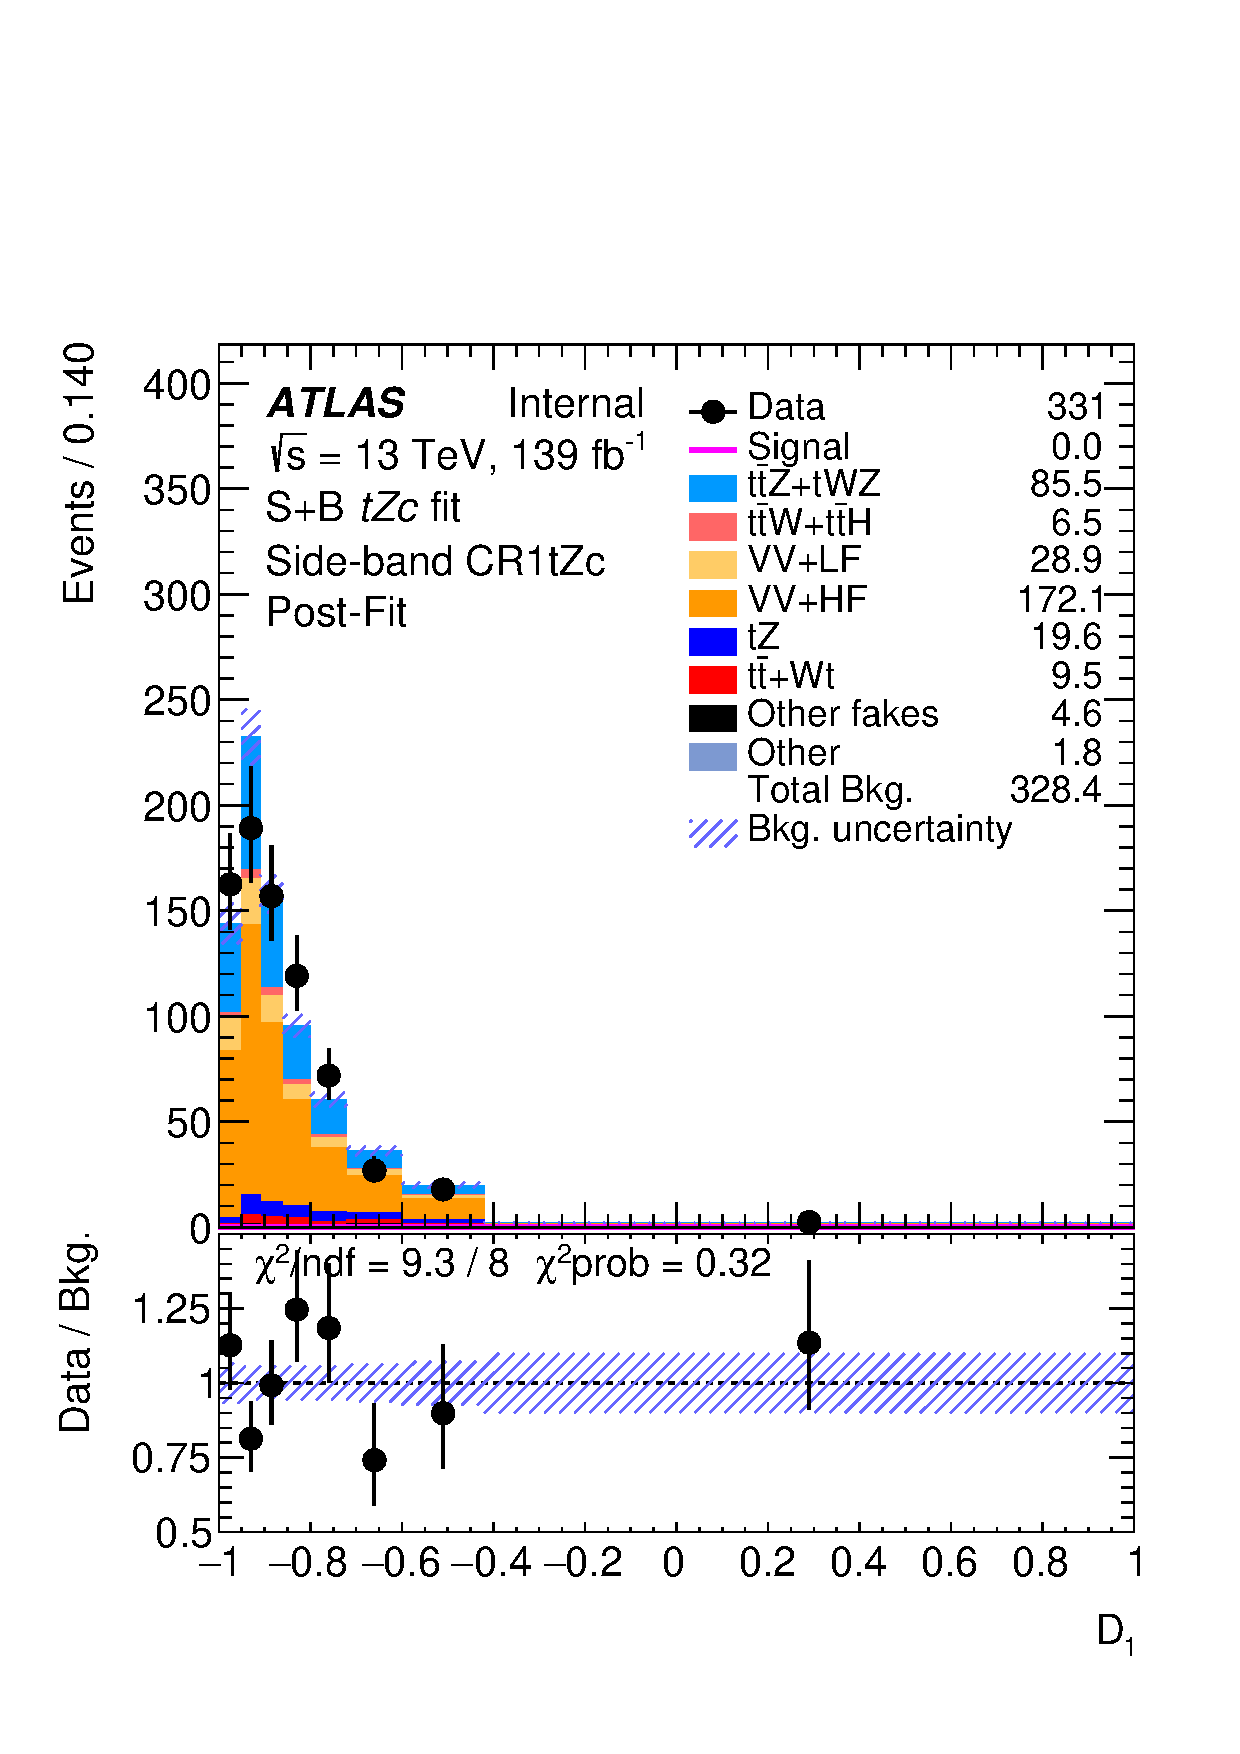
\includegraphics[width=.45\textwidth]{Chapters/CH8/figures/SPLUSB_CRSR_UsingDL1rcFullSys/Plots/SBCR1_postFit} \\
		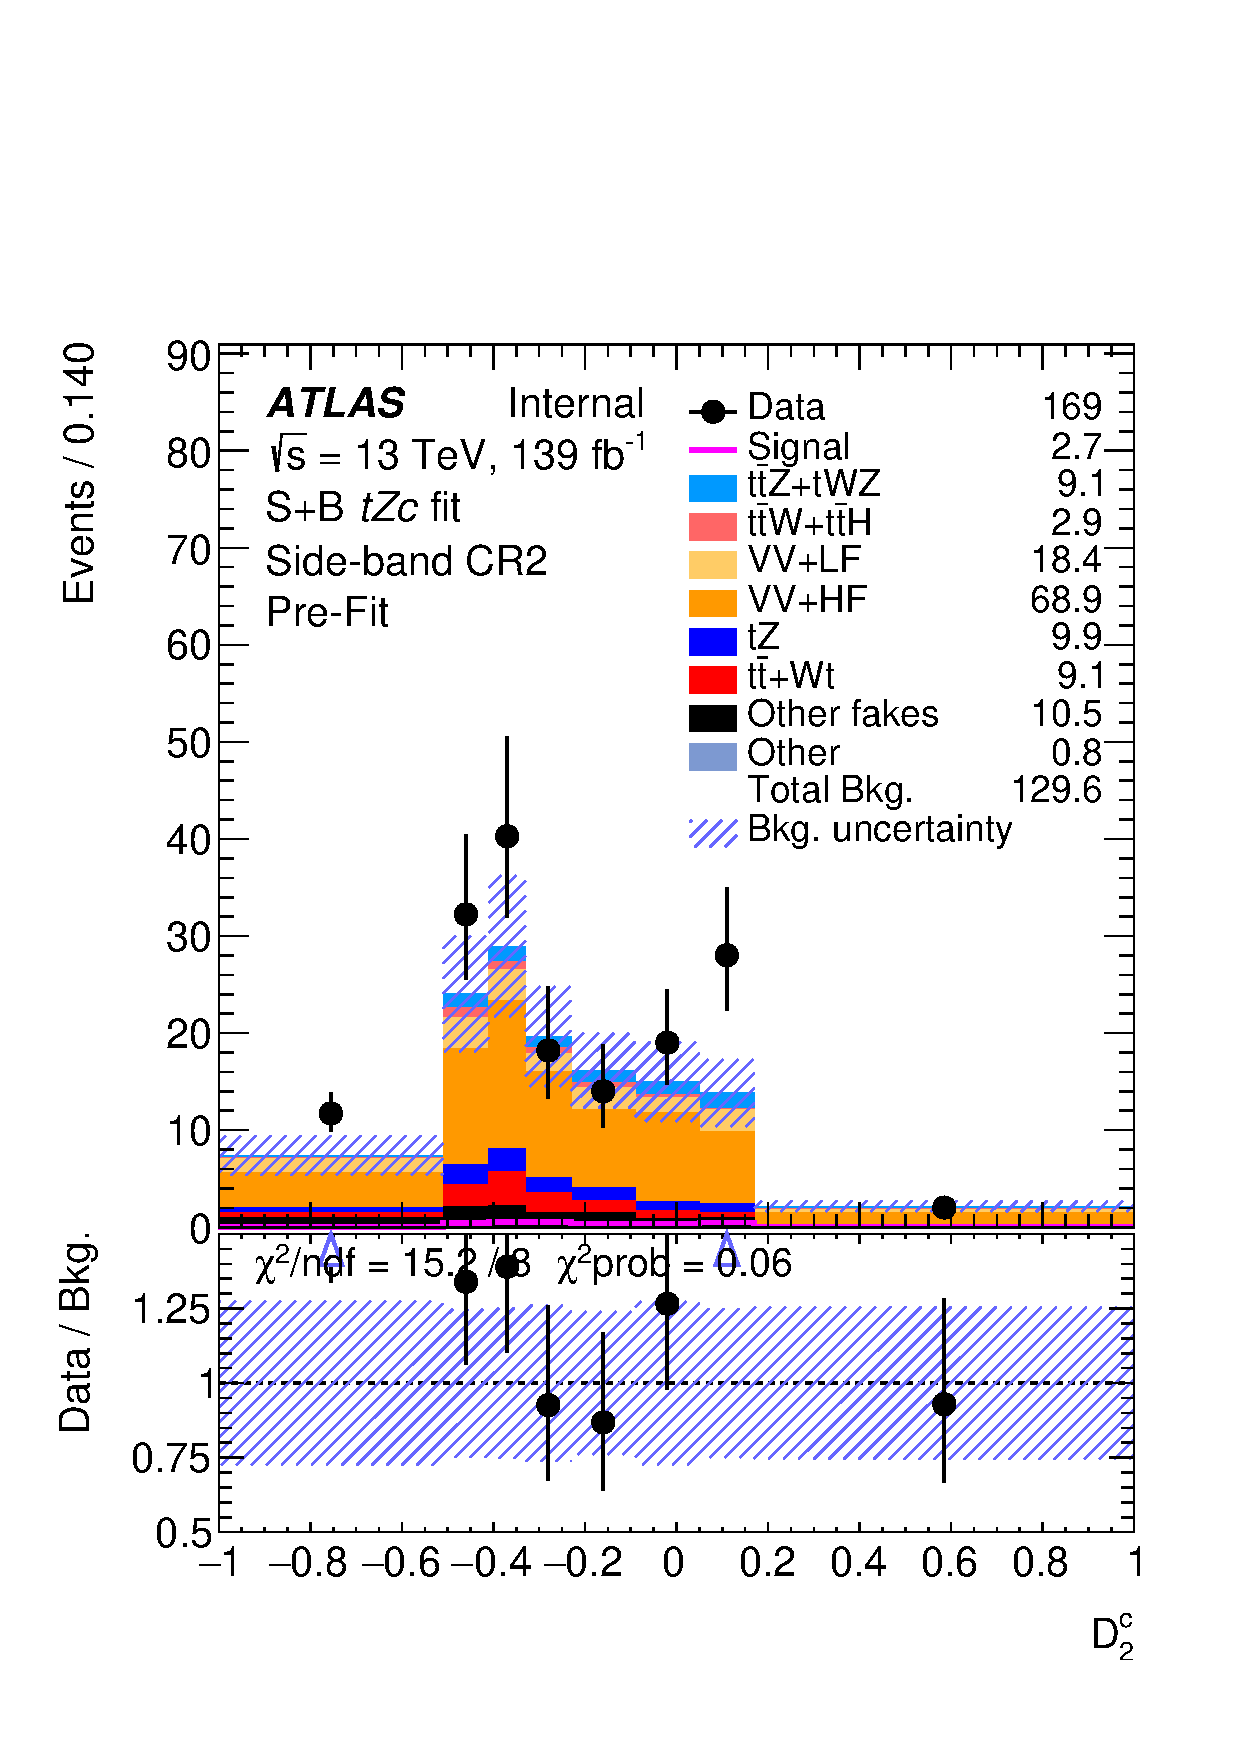
\includegraphics[width=.45\textwidth]{Chapters/CH8/figures/SPLUSB_CRSR_UsingDL1rcFullSys/Plots/SBCR2} &
		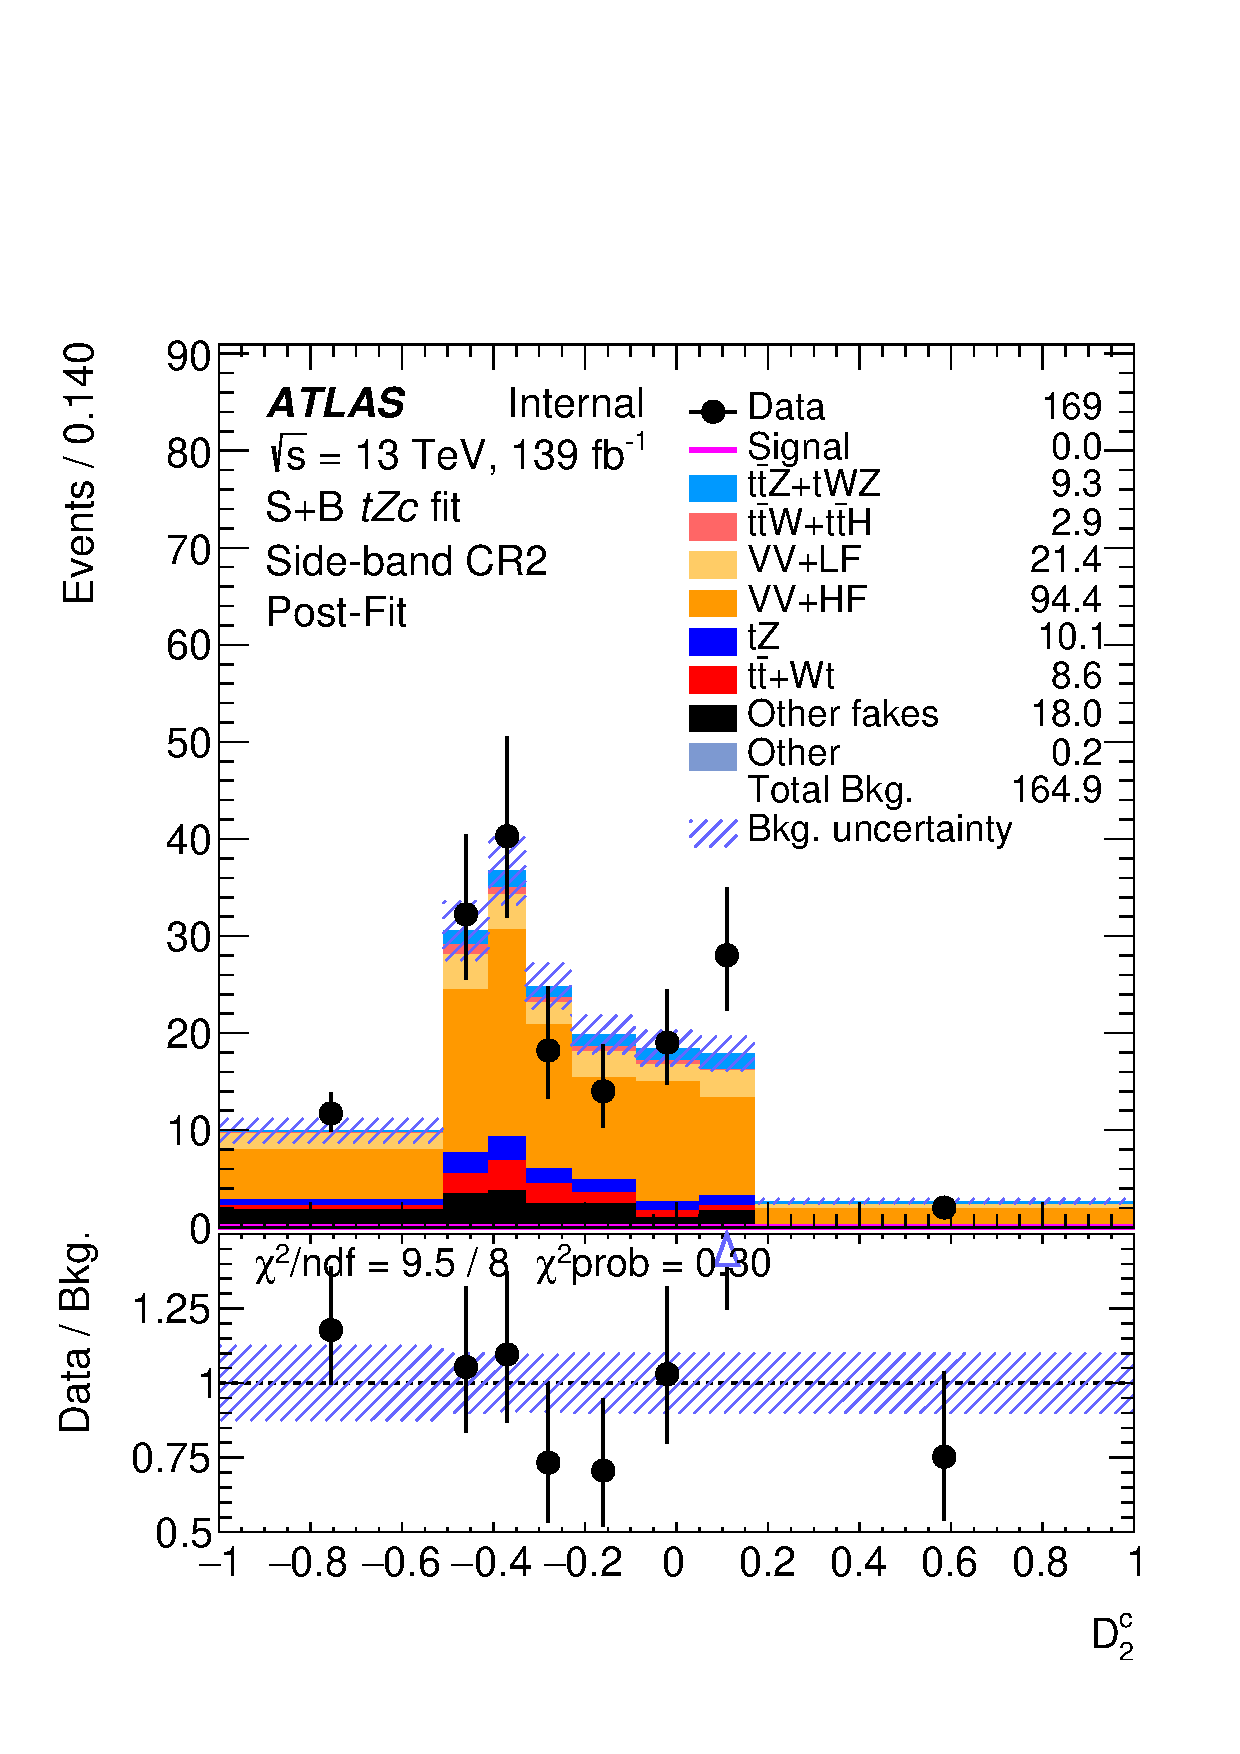
\includegraphics[width=.45\textwidth]{Chapters/CH8/figures/SPLUSB_CRSR_UsingDL1rcFullSys/Plots/SBCR2_postFit} \\
	\end{tabular}
	\caption{Pre-fit (left) and post-fit (right) BDTG output distributions in the side-band CRs for the S+B \tZc fit in SRs+CRs with realistic Asimov.
		\ErrStatSys
	}%
	\label{fig:stat:tzc:splusb:crsr:crplots:1}
\end{figure}

\begin{figure}[htbp]
	\centering
	\begin{tabular}{cc}
		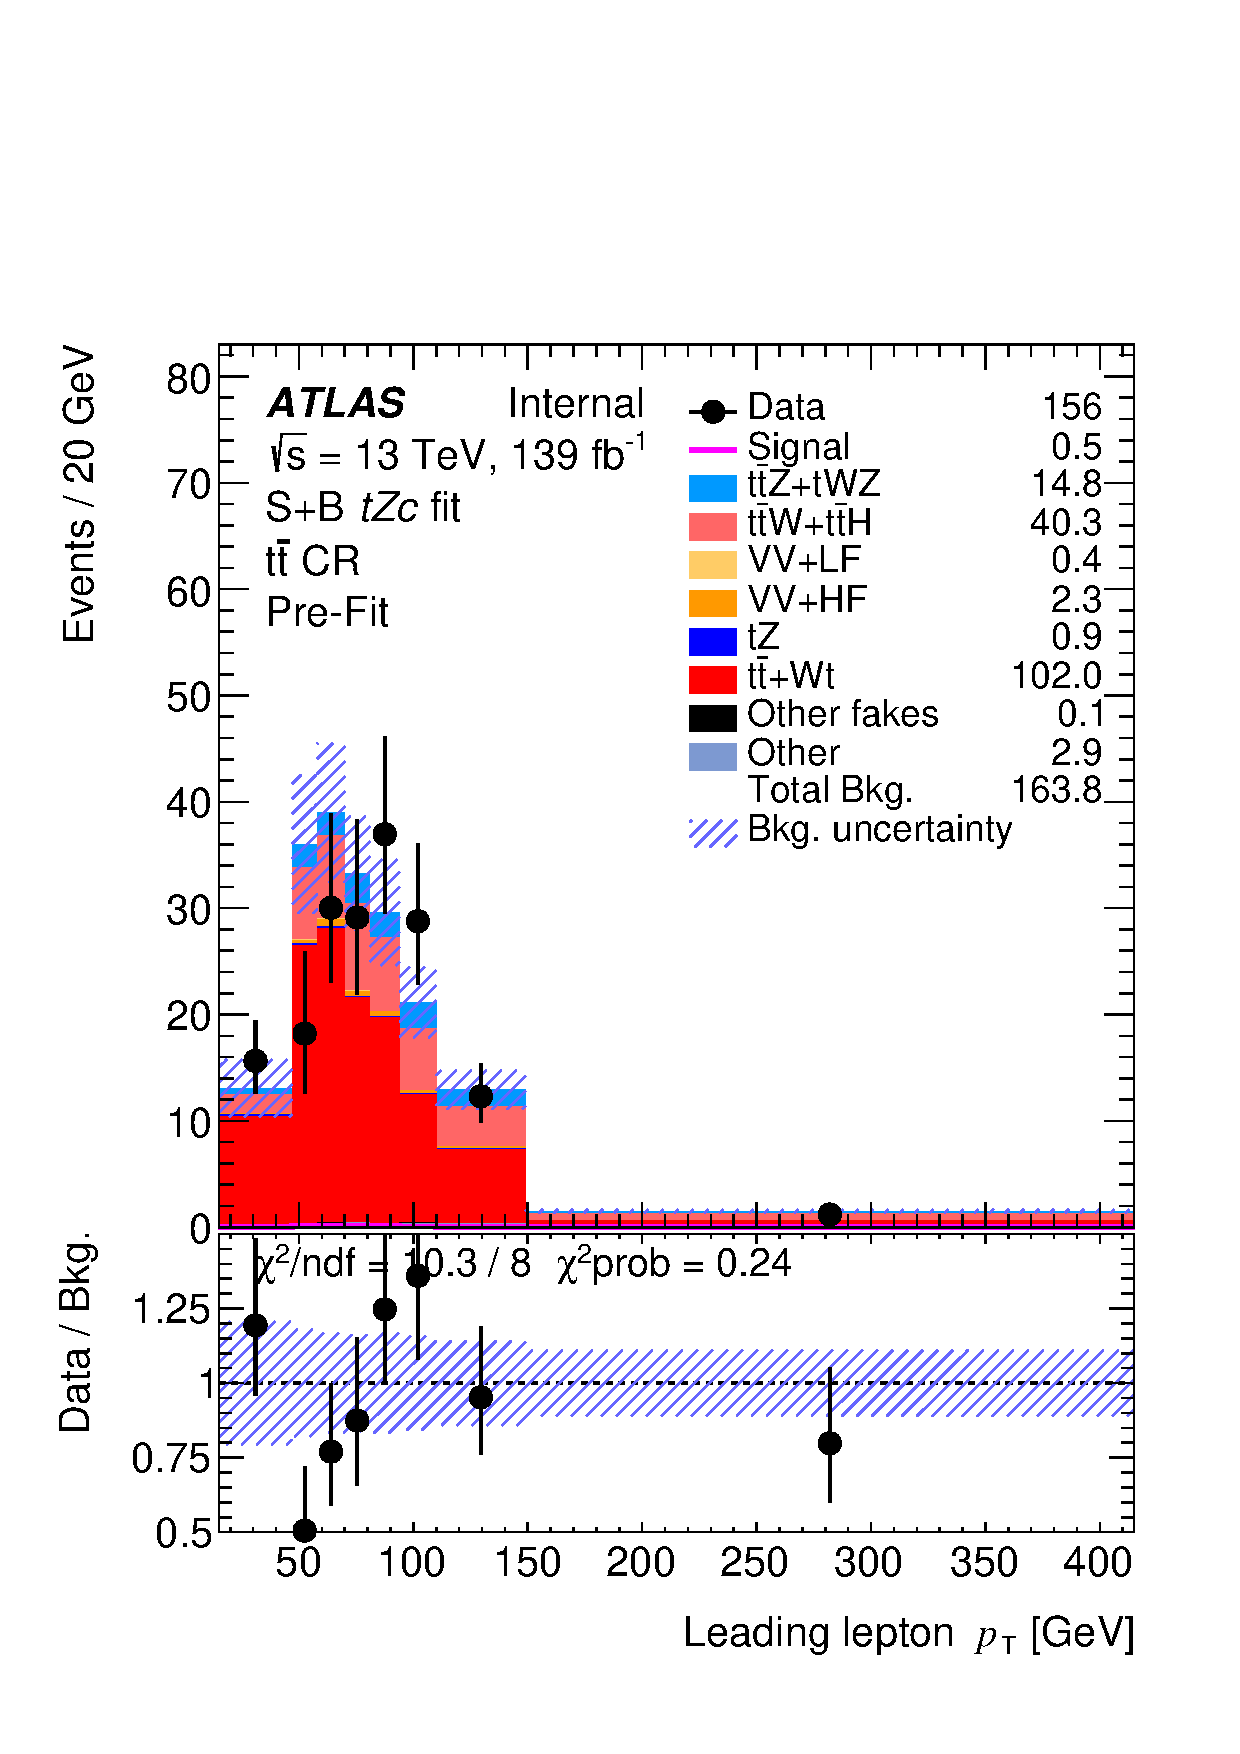
\includegraphics[width=.45\textwidth]{Chapters/CH8/figures/SPLUSB_CRSR_UsingDL1rcFullSys/Plots/TTCR} &
		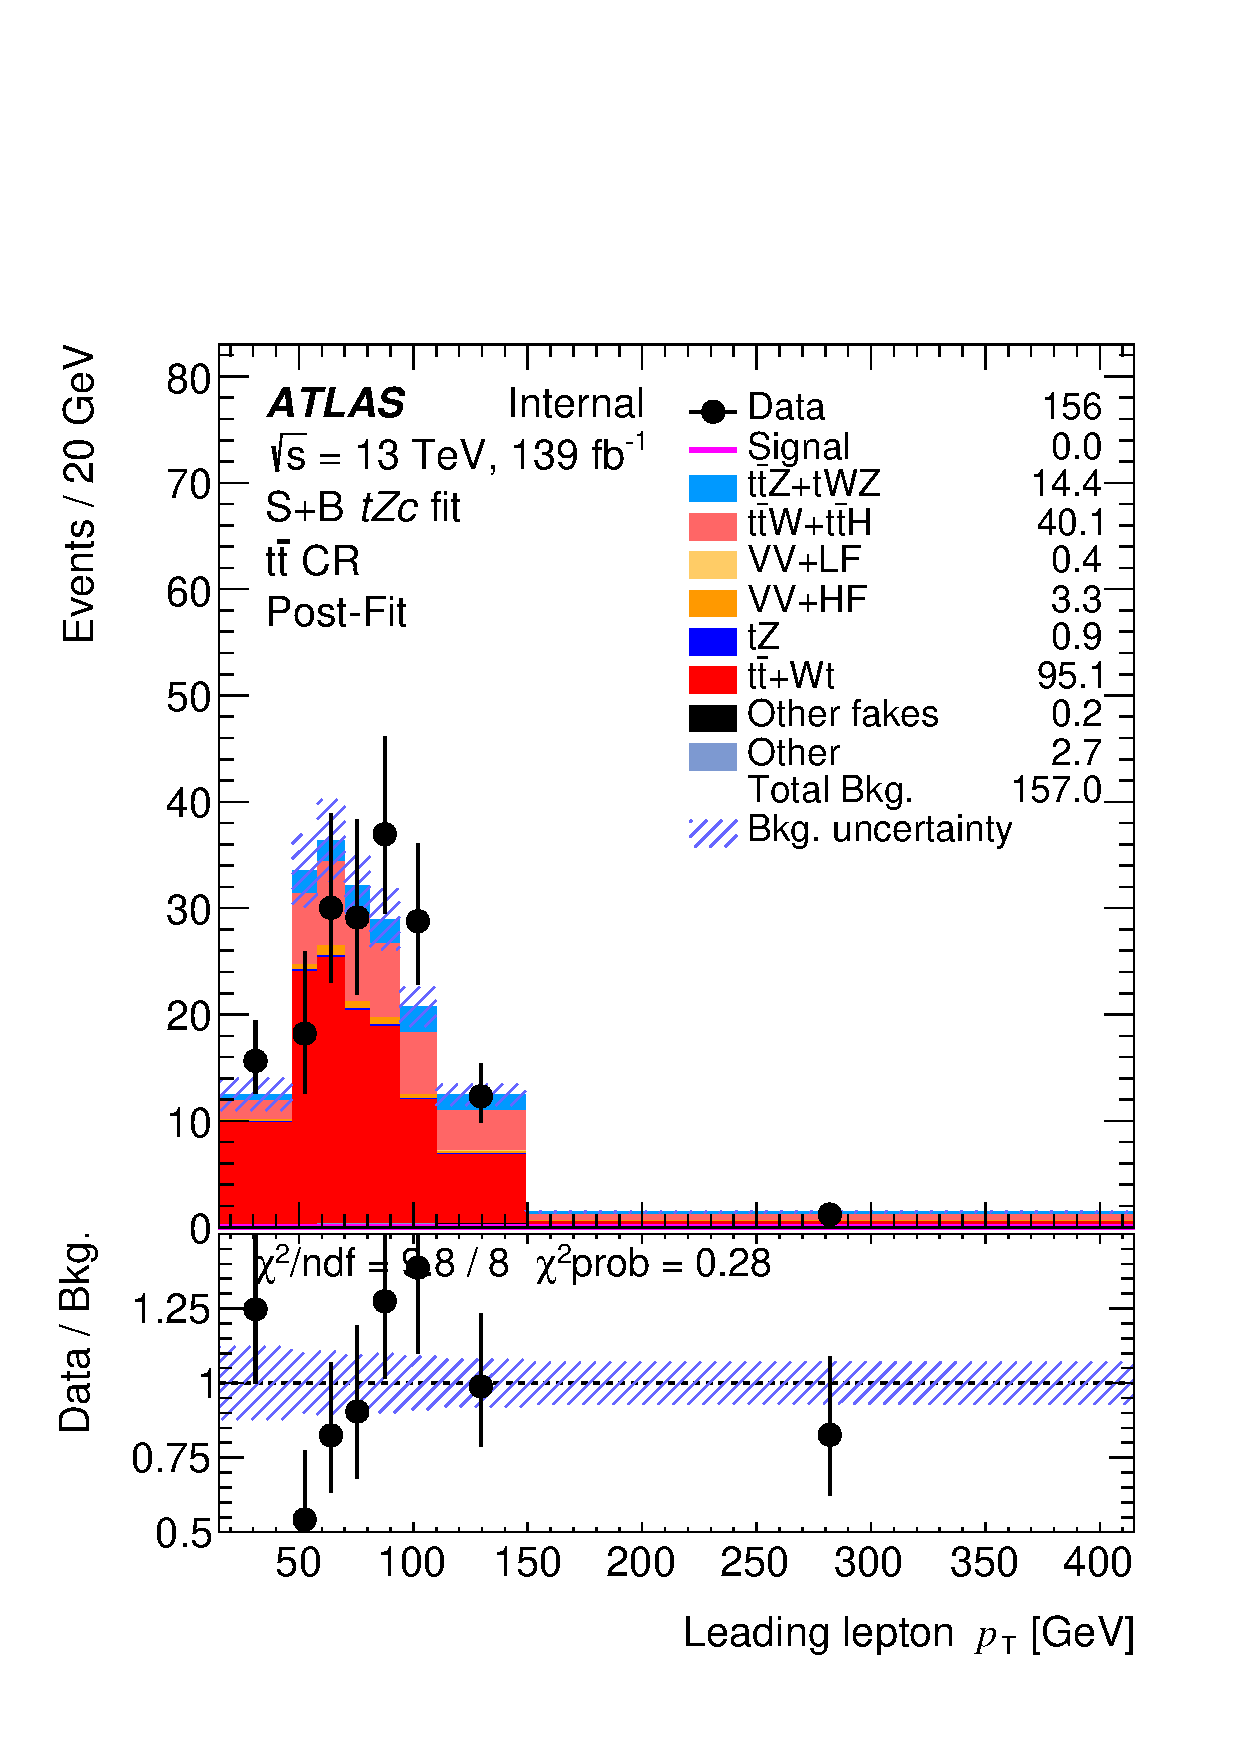
\includegraphics[width=.45\textwidth]{Chapters/CH8/figures/SPLUSB_CRSR_UsingDL1rcFullSys/Plots/TTCR_postFit} \\
		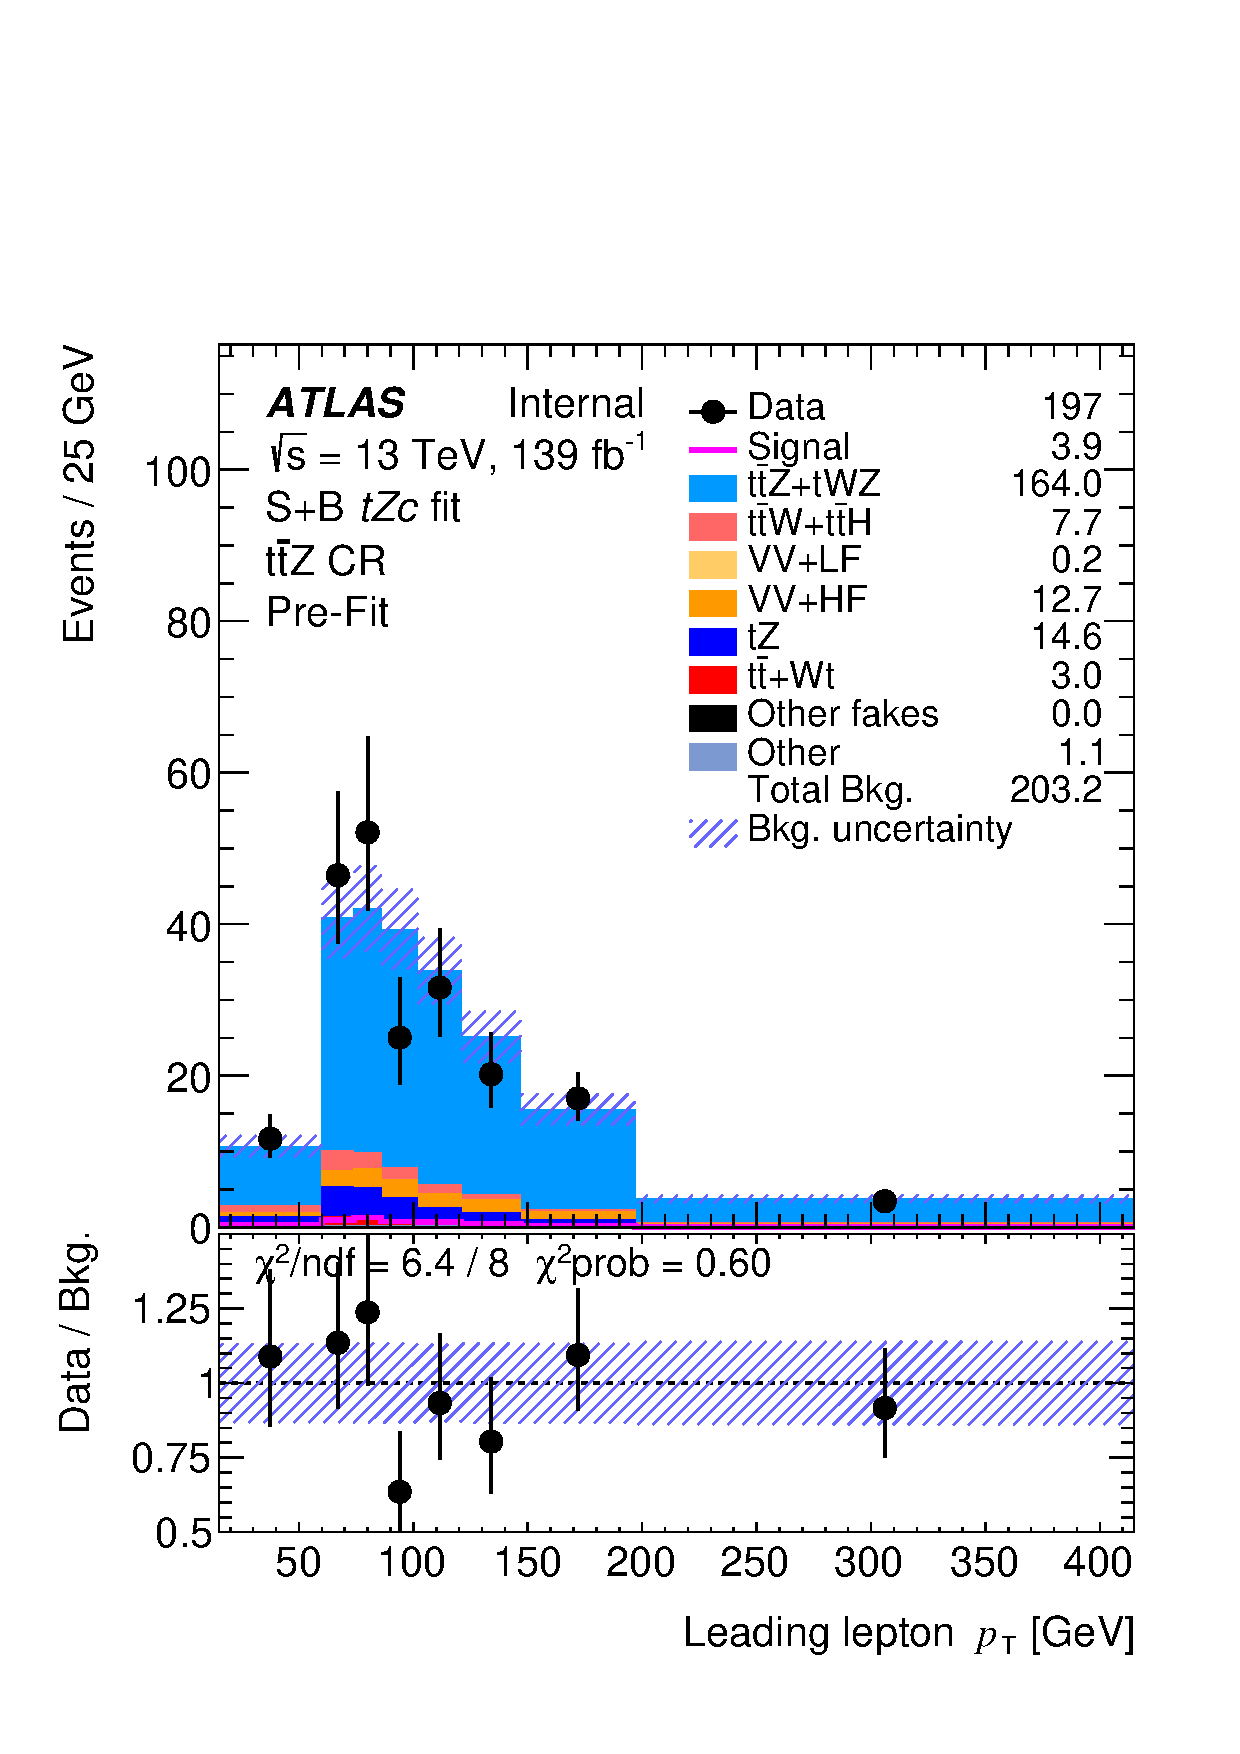
\includegraphics[width=.45\textwidth]{Chapters/CH8/figures/SPLUSB_CRSR_UsingDL1rcFullSys/Plots/TTZCR} &
		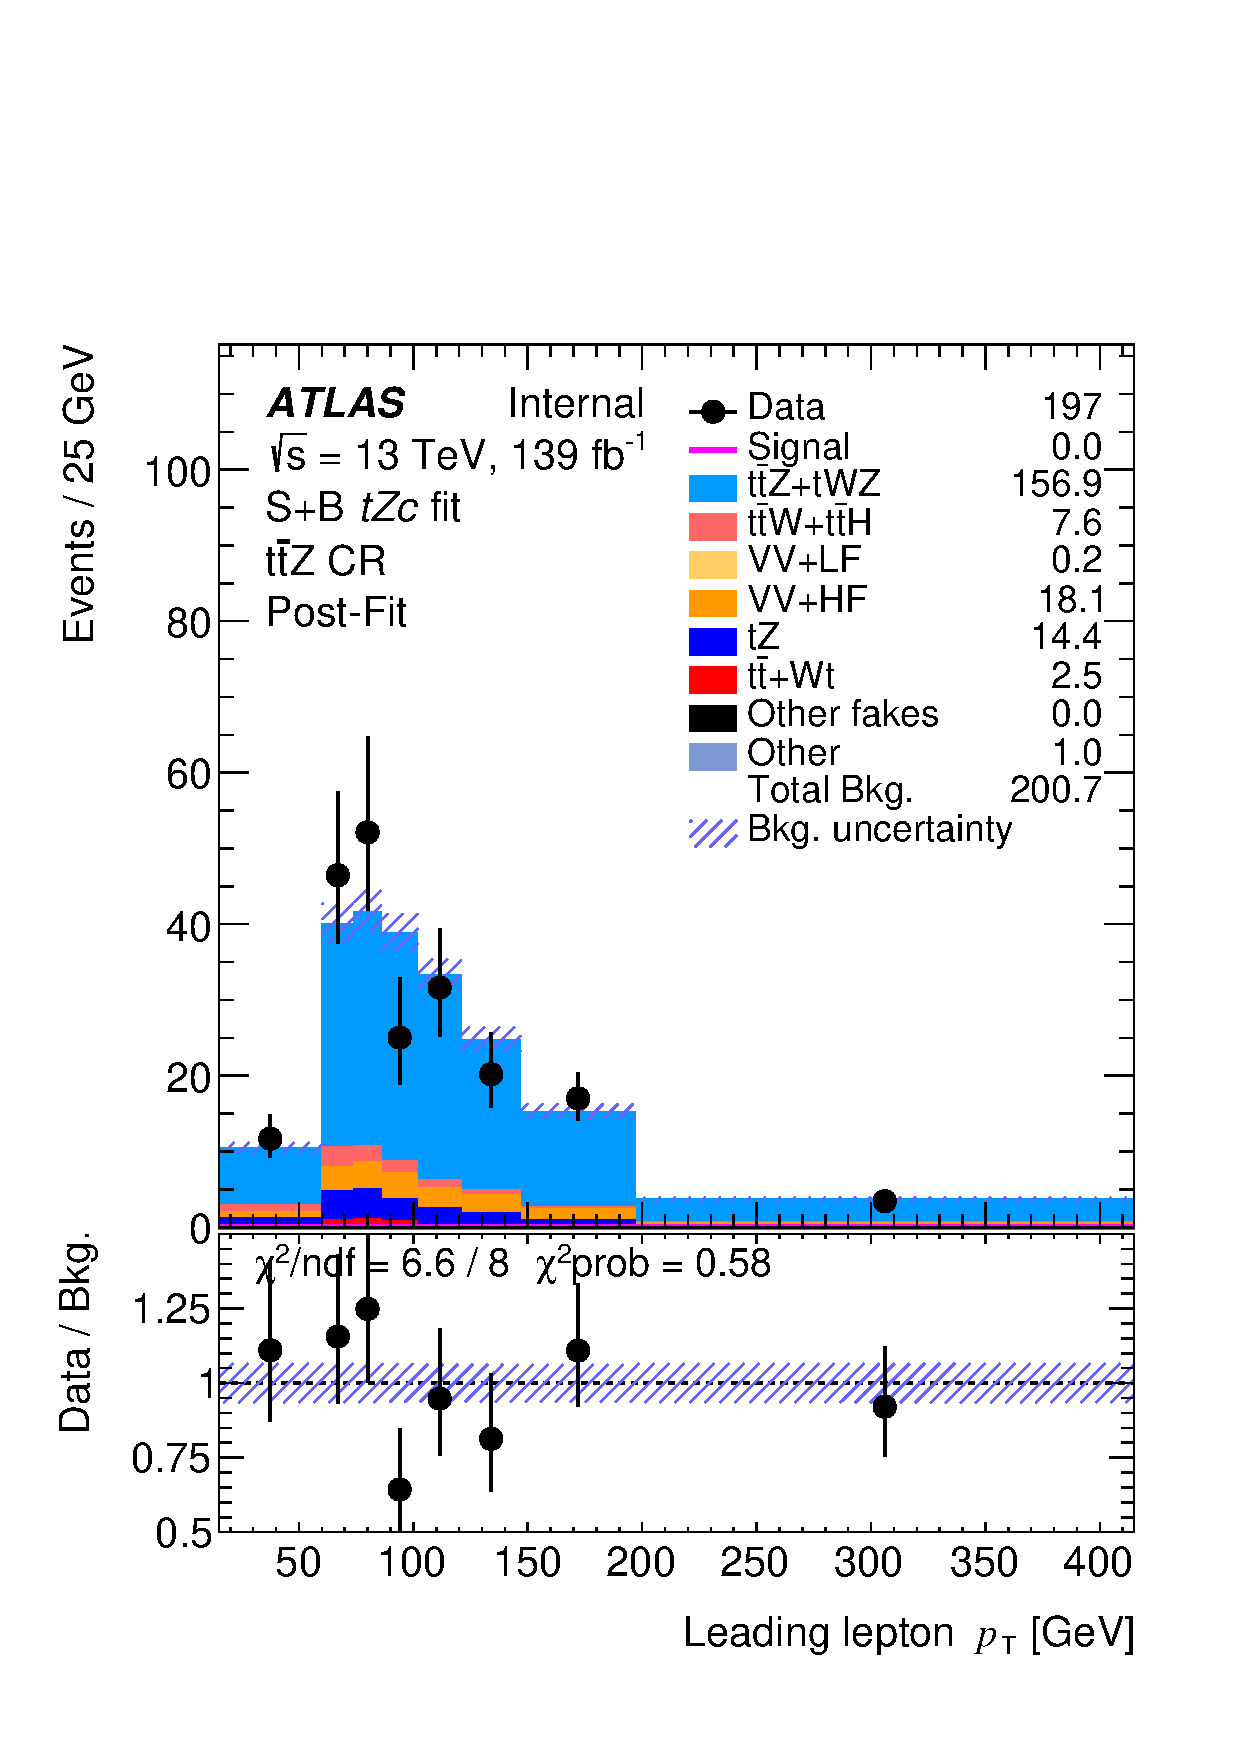
\includegraphics[width=.45\textwidth]{Chapters/CH8/figures/SPLUSB_CRSR_UsingDL1rcFullSys/Plots/TTZCR_postFit} \\
	\end{tabular}
	\caption{Pre-fit (left) and post-fit (right) leading lepton \pt distributions in the \ttbar and \ttZ CRs for the S+B \tZc fit in SRs+CRs with realistic Asimov.
		\ErrStatSys
	}%
	\label{fig:stat:tzc:splusb:crsr:crplots:2}
\end{figure}

\clearpage
\section{Results}
\label{sec:stat:tzc}
From the fits described in this chapter, in particular the
signal+background fits in SRs+CRs with the realistic Asimov datasets in \Cref{sec:stat:tzc:splusb:crsr},
expected limits on the branching ratios of
$\Pqt\rightarrow\PZ\Pqc$ are extracted. \\
In Table \ref{tab:limits:comparison} is also possible to estimate the impact of the \Pqc-tagging using \DLrc or SMT (presented in \Cref{chapter:charm_tag}) on the analysis comparing the results without using none of these techniques (called 'Baseline').\\
The improvement obtained using SMT is around 2\%, while using \DLrc is around 10\%.
\begin{table}[htbp]
	\centering
	\begin{tabular}{c|c|c}
		\toprule
		\multicolumn{3}{c}{Expected limits on BR $\Pqt\rightarrow\PZ\Pqc$ }\\
		\toprule
		 \textbf{Baseline [$ \times 10^{-5}$]}          & \textbf{Using SMT [$ \times 10^{-5}$]}			& \textbf{Using \DLrc} \\
		 \midrule
		 $10.67 $ 	& $ 10.43 $   & $  9.55 $\\
		\bottomrule
	\end{tabular}
	\caption{ Expected limits on the branching ratios of $\Pqt\rightarrow\PZ\Pqc$. 
					Results using \DLrc, SMT and none of them are reported to estimate the impact of these techniques on the analysis.  }%
	\label{tab:limits:comparison}
\end{table}
\\The expected limits, together
with statistical only limits and the expected limits from the previous ATLAS
analysis~\cite{TOPQ-2017-06}, are reported in
\cref{tab:results:limits}.\\
The overall impact of systematics on the expected limit is 22\%.\\
The limit from the previous analysis is improved by a factor of 2.3 for the \tZc coupling.
\begin{table}[htbp]
	\centering
	\begin{tabular}{lccc}
		\toprule
		\textbf{Limits} & \textbf{$-1\sigma$} & \textbf{Expected} & \textbf{$+1\sigma$} \\
		\midrule
		BR $\Pqt\rightarrow\PZ\Pqc$ \cite{TOPQ-2017-06} & \SI{2.2e-4}{} & \SI{3.2e-4}{} & \SI{4.6e-4}{} \\
		BR $\Pqt\rightarrow\PZ\Pqc$  (stat. only)                 & \SI{5.3e-5}{} & \SI{7.4e-5}{} & \SI{10.5e-5}{} \\
		BR $\Pqt\rightarrow\PZ\Pqc$                                    & \SI{6.9e-5}{} & \SI{9.6e-5}{} & \SI{13.8e-5}{} \\		
		\bottomrule
	\end{tabular}
	\caption{
	Expected limits on the branching ratios of $\Pqt\rightarrow\PZ\Pqc$.
	Expected limit from \cite{TOPQ-2017-06} is also included for reference.
}%
\label{tab:results:limits}
\end{table}

